\documentclass[
	12pt,
%	%BCOR=5mm,
	DIV=14,
	headinclude=on,
	footinclude=off,
	parskip=half,
	bibliography=totoc,
	listof=entryprefix,
	toc=listof,
	pointlessnumbers,
	plainfootsepline]{scrreprt}
	
	%\usepackage[paperwidth=210mm, paperheight=245mm, top=25mm, bottom=20mm, left=25mm,	right=25mm,]{geometry}

%\usepackage[onehalfspacing]{setspace}

% Theorem

%	Konfigurationsdatei einziehen
% !TEX root =  master.tex
% 		HYPERREF
%
\usepackage[
hidelinks=true % keine roten Markierungen bei Links
]{hyperref}

% \newcommand*{\Kapitel}{../Kapitel}


\newcommand{\TitelDerArbeit}[1]{\def\DerTitelDerArbeit{#1}\hypersetup{pdftitle={#1}}}
\newcommand{\AutorDerArbeit}[1]{\def\DerAutorDerArbeit{#1}\hypersetup{pdfauthor={#1}}}
\newcommand{\ZweiterAutorDerArbeit}[1]{\def\DerZweiteAutorDerArbeit{#1}\hypersetup{pdfauthor={#1}}}
\newcommand{\DritterAutorDerArbeit}[1]{\def\DerDritteAutorDerArbeit{#1}\hypersetup{pdfauthor={#1}}}
\newcommand{\Firma}[1]{\def\DerNameDerFirma{#1}}
\newcommand{\Kurs}[1]{\def\DieKursbezeichnung{#1}}



%		FONT AND INPUT ENCODING
%
\usepackage[T1]{fontenc}
\usepackage[utf8]{inputenc}

%		CALCULATIONS
%
\usepackage{calc} % Used for extra space below footsepline

%		LANGUAGE SETTINGS
%
%\usepackage[ngerman]{babel} 	% German language
%\usepackage[german=quotes]{csquotes} 	% correct quotes using \enquote{}

\usepackage[english]{babel}   % For english language
\usepackage{csquotes} 	% Richtiges Setzen der Anführungszeichen mit \enquote{}


%		BIBLIOGRAPHY SETTINGS
%
%\usepackage[backend=biber, autocite=footnote, style=authortitle-ibid, dashed=false,ibidtracker=context]{biblatex} 	%Use Author-Year-Cites with footnotes
 \usepackage[backend=biber, autocite=inline, style=ieee, , sorting=nty, dashed=false]{biblatex} 	% Use IEEE-Style (e.g. [1])
% \usepackage[backend=biber, autocite=inline, style=alphabetic]{biblatex} 	% Use alphabetic style (e.g. [TGK12])
%%%% APA/Harvard-Style (bitte die nächten zwei Zeilen auskommentieren)
%\usepackage[backend=biber, style=apa]{biblatex} 	
%\DeclareLanguageMapping{german}{german-apa}

\DefineBibliographyStrings{ngerman}{  %Change u.a. to et al. (german only!)
	andothers = {{et\,al\adddot}},
}
\DefineBibliographyStrings{ngerman}{%
	urlseen = {Last accessed},
}

%%% Uncomment the following lines to support hard URL breaks in bibliography 
%\apptocmd{\UrlBreaks}{\do\f\do\m}{}{}
%\setcounter{biburllcpenalty}{9000}% Kleinbuchstaben
%\setcounter{biburlucpenalty}{9000}% Großbuchstaben


\setlength{\bibparsep}{\parskip}		%add some space between biblatex entries in the bibliography
\addbibresource{bibliography.bib}	%Add file bibliography.bib as biblatex resource


%		FOOTNOTES 
%
% Count footnotes over chapters
\usepackage{chngcntr}
\counterwithout{footnote}{chapter}


%	ACRONYMS
%%%
%%% WICHTIG: Installieren Sie das neueste Acronyms-Paket!!!
%%%
\makeatletter
\usepackage[nolist]{acronym}
\@ifpackagelater{acronym}{2015/03/20}
{%
	\renewcommand*{\aclabelfont}[1]{\textbf{\textsf{\acsfont{#1}}}}
}%
{%
}%
\makeatother

%		LISTINGS
\usepackage{listings}	%Format Listings properly
\usepackage{xcolor}
\usepackage{bera}% optional: just to have a nice mono-spaced font
%\renewcommand{\lstlistingname}{Quelltext} 
\renewcommand{\lstlistlistingname}{Quelltextverzeichnis}

\lstset{numbers=left,
	numberstyle=\tiny,
	captionpos=b,
	basicstyle=\ttfamily\small}

\colorlet{punct}{red!60!black}
\definecolor{background}{HTML}{EEEEEE}
\definecolor{delim}{RGB}{20,105,176}
\colorlet{numb}{magenta!60!black}

\lstdefinelanguage{json}{
	basicstyle=\normalfont\ttfamily,
	numbers=left,
	numberstyle=\scriptsize,
	stepnumber=1,
	numbersep=8pt,
	showstringspaces=false,
	breaklines=true,
	frame=lines,
	backgroundcolor=\color{background},
	literate=
	*{0}{{{\color{numb}0}}}{1}
	{1}{{{\color{numb}1}}}{1}
	{2}{{{\color{numb}2}}}{1}
	{3}{{{\color{numb}3}}}{1}
	{4}{{{\color{numb}4}}}{1}
	{5}{{{\color{numb}5}}}{1}
	{6}{{{\color{numb}6}}}{1}
	{7}{{{\color{numb}7}}}{1}
	{8}{{{\color{numb}8}}}{1}
	{9}{{{\color{numb}9}}}{1}
	{:}{{{\color{punct}{:}}}}{1}
	{,}{{{\color{punct}{,}}}}{1}
	{\{}{{{\color{delim}{\{}}}}{1}
	{\}}{{{\color{delim}{\}}}}}{1}
	{[}{{{\color{delim}{[}}}}{1}
	{]}{{{\color{delim}{]}}}}{1},
}

%		EXTRA PACKAGES
\usepackage{lipsum}    %Blindtext
\usepackage{graphicx} % use various graphics formats
\usepackage[german]{varioref} 	% nicer references \vref
\usepackage{caption}	%better Captions
\captionsetup[table]{position=bottom} 
\usepackage{booktabs} %nicer Tabs
\usepackage{array}
\usepackage{pdfpages} 
\usepackage{algpseudocode}% http://ctan.org/pkg/algorithmicx
%\newcolumntype{P}[1]{>{\raggedright\arraybackslash}p{#1}}
\usepackage{tikz}
\usepackage{amssymb}

\usepackage{multirow}

\newcommand\MyBox[2]{
	\fbox{\lower0.75cm
		\vbox to 1.7cm{\vfil
			\hbox to 1.7cm{\hfil\parbox{1.4cm}{#1\\#2}\hfil}
			\vfil}%
	}%
}



%chapter settings
\usepackage{etoolbox}

%		ALGORITHMS
\usepackage{algorithm}
\usepackage{amsmath}
\usepackage{algpseudocode}
\usepackage{soul}
\usepackage{bchart}
\renewcommand{\listalgorithmname}{Algorithmenverzeichnis}
\floatname{algorithm}{Algorithmus}


%		FONT SELECTION: Entweder Latin Modern oder Times / Helvetica
\usepackage{lmodern} %Latin modern font
\usepackage{tabularx}
%\usepackage{mathptmx}  %Helvetica / Times New Roman fonts (2 lines)
%\usepackage[scaled=.92]{helvet} %Helvetica / Times New Roman fonts (2 lines)

%		PAGE HEADER / FOOTER
%	    Warning: There are some redefinitions throughout the master.tex-file!  DON'T CHANGE THESE REDEFINITIONS!
\RequirePackage{scrlfile}
\ReplacePackage{scrpage2}{scrlayer-scrpage}
\RequirePackage[automark,headsepline,footsepline]{scrpage2}
\pagestyle{scrheadings}
\renewcommand*{\pnumfont}{\upshape\sffamily}
\renewcommand*{\headfont}{\upshape\sffamily}
\renewcommand*{\footfont}{\upshape\sffamily}
\renewcommand{\chaptermarkformat}{}

\clearscrheadfoot

\ifoot[\rule{0pt}{\ht\strutbox+\dp\strutbox}Advanced Machine Learning]{\rule{0pt}{\ht\strutbox+\dp\strutbox}Advanced Machine Learning}
\ofoot[\rule{0pt}{\ht\strutbox+\dp\strutbox}\pagemark]{\rule{0pt}{\ht\strutbox+\dp\strutbox}\pagemark}

\ohead{\headmark}

\usepackage{chngcntr}
\counterwithout{figure}{chapter}
\counterwithout{table}{chapter}

%zeilenumbrüche
\setlength{\emergencystretch}{1em}

\usetikzlibrary{calc,trees,positioning,arrows,chains,shapes.geometric,%
	decorations.pathreplacing,decorations.pathmorphing,shapes,%
	matrix,shapes.symbols,quotes,angles,babel,calc}
\usepackage{tikz-qtree-compat,tikz-qtree}

\nocite{*}

\tikzset{
	>=stealth',
	punktchain/.style={
		rectangle, 
		rounded corners, 
		% fill=black!10,
		draw=black, very thick,
		text width=10em, 
		minimum height=3em, 
		text centered, 
		on chain},
	line/.style={draw, thick, <-},
	element/.style={
		tape,
		top color=white,
		bottom color=blue!50!black!60!,
		minimum width=8em,
		draw=blue!40!black!90, very thick,
		text width=10em, 
		minimum height=3.5em, 
		text centered, 
		on chain},
	every join/.style={->, thick,shorten >=1pt},
	decoration={brace},
	tuborg/.style={decorate},
	tubnode/.style={midway, right=2pt},
}


\definecolor{myblue}{RGB}{209, 216, 224}

\usepackage{amsthm}

\theoremstyle{plain}
\newtheorem{thm}{Theorem}[chapter] % reset theorem numbering for each chapter

\theoremstyle{definition}
\newtheorem{defn}[thm]{Definition} % definition numbers are dependent on theorem numbers
\newtheorem{exmp}[thm]{Example} % same for example numbers

\usepackage{epstopdf}

\makeatletter
\newcommand{\chapterauthor}[1]{%
	{\parindent0pt\vspace*{-35pt}%
		\linespread{1.1}\large\scshape#1%
		\par\nobreak\vspace*{5pt}}
	\@afterheading%
}
\makeatother

\makeatletter
\newcommand{\sectionauthor}[1]{%
	{\parindent0pt\vspace*{-20pt}%
		\linespread{1.1}\large\scshape#1%
		\par\nobreak\vspace*{5pt}}
	\@afterheading%
}
\makeatother

\makeatletter
\newcommand{\subsubsectionauthor}[1]{%
	{\parindent0pt\vspace*{-20pt}%
		\linespread{1.1}\scshape#1%
		\par\nobreak\vspace*{5pt}}
	\@afterheading%
}
\makeatother

\addbibresource{bibliography.bib}


\begin{document}

% Disable listing with chapter numbers
\counterwithout{lstlisting}{chapter}
\counterwithout{equation}{chapter}
% CHAPTER CHANGES
\renewcommand*{\chapterheadstartvskip}{\vspace*{0cm}}
\renewcommand*{\chapterheadendvskip}{\vspace{1cm}}


\makeatletter
\patchcmd{\scr@startchapter}{\if@openright\cleardoublepage\else\clearpage\fi}{}{}{}
\makeatother

\TitelDerArbeit{SIIM-FISABIO-RSNA COVID-19 Detection}
\AutorDerArbeit{Tobias Richstein (3596554)}
\ZweiterAutorDerArbeit{Julian Seibel (3601340)}
\DritterAutorDerArbeit{Torben Krieger (3663391)}
\begin{titlepage}
\begin{minipage}{\textwidth}
		\vspace{-2cm}
		\centering
		 
\includegraphics[scale=0.35]{img/uni_blacksmall.png}
\end{minipage}
\vspace{6em}
\sffamily
\begin{center}
	\textsf{\large{}Ruprecht-Karls-Universität \\ Heidelberg}\\[2em]
	\textsf{\textbf{\Large{}Final project report}}\\[3mm]
	\textsf{\textbf{Advanced Machine Learning}} \\[3mm] \textsf{Prof. Dr. Köthe} \\[1.5cm]
	\textsf{\textbf{\Large{}\DerTitelDerArbeit}}\\[1.5cm]

	
	\vspace{3em}
	%\textsf{\Large{Sperrvermerk}}
\vfill

\begin{minipage}{\textwidth}

\begin{tabbing}
	Wissenschaftlicher Betreuer: \hspace{0.85cm}\=\kill
	Authors: \> \DerAutorDerArbeit \\ \> \DerZweiteAutorDerArbeit \\ \>  \DerDritteAutorDerArbeit \\ [1.5mm]
	Field of Studies: \> M. Sc. Applied Computer Science \\[1.5mm]
	Period: \> Summer term 2021
\end{tabbing}
\end{minipage}

\end{center}

\end{titlepage}

\pagenumbering{Roman} % Römische Seitennummerierung
\normalfont

%--------------------------------
% Verzeichnisse - nicht benötige Verzeichnisse bitte auskommentieren / löschen.
%--------------------------------

%Sperrvermerk
%\input{Kapitel/sperrvermerk.tex}

%\input{Kapitel/widmung.tex}

%	Kurzfassung
%\chapter*{Kurzfassung}
\begingroup
\begin{table}[h!]
\setlength\tabcolsep{0pt}
\begin{tabular}{p{3.7cm}p{11.7cm}}
Titel: & \DerTitelDerArbeit \\
Verfasser: & \DerAutorDerArbeit \\
\end{tabular}
\end{table}
\endgroup



%	Inhaltsverzeichnis
\tableofcontents

%	Abbildungsverzeichnis
%\listoffigures

%	Tabellenverzeichnis
%\listoftables

%	Listingsverzeichnis
 %\lstlistoflistings

% 	Algorithmenverzeichnis
 %\listofalgorithms

% 	Abkürzungsverzeichnis (siehe Datei acronyms.tex!)

\begin{acronym}[]
	\acro{CNN}{Convolutional Neural Network}
	\acro{IoU}{Intersection over Union}
	\acro{mAP}{mean Average Precision}
	\acro{R-CNN}{Region Based CNN}
	\acro{SGD}{Stochastic Gradient Descent}
	\acro{CAD}{Computer Aided detection and diagnosis}
	\acro{CIoU}{Complete-IoU}
	\acro{SVM}{Support Vector Machine}
	\acro{YOLO}{You only look once}
	\acro{RT-PCR}{Real‐Time reverse transcription Polymerase Chain Reaction}
	\acro{CT}{Computed Tomography}
	\acro{MSE}{mean squared error}
	\acro{GIoU}{Generalized Intersection over Union}
	\acro{DIoU}{Distance Intersection over Union}
	\acro{NIH}{National Institutes of Health}
	\acro{RSNA}{Radiological Society of North America}
	\acro{CXR}{Chest X-Ray}
	\acro{PNG}{Portable Network Graphics}
	\acro{COCO}{Common Objects in Context}
\end{acronym}


%--------------------------------
% Start des Textteils der Arbeit
%--------------------------------
\clearpage
\ihead{\chaptername~\thechapter} % Neue Header-Definition
\pagenumbering{arabic}  % Arabische Seitenzahlen

%	Anleitungs-Datei anleitung.tex einziehen. Auf diese Weise sollten Sie versuchen, für jedes einzelne
% Kapitel eine eigene Datei anzulegen und mittels input-Kommando einzuziehen.
%% !TEX root =  master.tex
\chapter{Gebrauchsanleitung}

\section{Übersicht über die Vorlage}
Die Vorlage wurde im UTF-8 Encoding erstellt. Sollten daher z.\,B. Umlaute in Ihrem \LaTeX-Editor nicht korrekt dargestellt werden, überprüfen Sie bitte die Encoding-Einstellungen des Editors. In seltenen Fällen müssen Sie die Vorlage danach noch einmal neu in den Editor einbinden. 
Die Vorlage beinhaltet die folgenden, in Tabelle \vref{tab:dateien} aufgelisteten Dateien: 
\begin{table}[h!]
	\centering
\begin{tabular}{lp{10cm}}
	\textbf{Dateiname} & \textbf{Beschreibung}\\\toprule
	\texttt{master.tex} & Die Hauptdatei. Alle anderen Dateien werden von dieser Datei eingezogen. \\
	\texttt{abstract.tex} & Die Kurzfassung der Arbeit. \\	
	\texttt{config.tex} & Konfigurationseinstellungen 	 der einzelnen Pakete\\
	\texttt{acronyms.tex} & Definition von Abkürzungen. \\
	\texttt{titlepage.tex} & Titelseite der Arbeit. \textbf{Bitte Anpassen!}\\
	\texttt{anleitung.tex} & Diese Anleitung\\ 
	\texttt{bibliography.bib}&  Die Literaturdatenbank -- hier können Sie die verwendete Literatur einpflegen.\\
	\texttt{ewerkl.tex} & Ehrenwörtliche Erklärung. \textbf{Bitte Anpassen!}\\
	\texttt{appendix.tex} & Anhang bzw. Anhänge \\\bottomrule
\end{tabular}
\caption{\label{tab:dateien}Übersicht über die Dateien der Vorlage}
\end{table}

Es werden -- unter anderem -- die folgenden Zusatzpakete von dieser Vorlage eingezogen und sollten daher in aktuellen Versionen installiert sein: 
\begin{itemize}
	\item\texttt{KOMA-Script} bzw. die Dokumentenklasse \texttt{scrreprt}
	\item\texttt{hyperref} für PDF-Informationen und Links 
	\item \texttt{babel} für länderspezifische Einstellungen
	\item \texttt{csquotes} für sprachabhängige Anführungszeichen (Befehl: \texttt{\textbackslash enquote})
	\item \texttt{acronym} für das Erstellen des Abkürzungsverzeichnisses 
	\item \texttt{booktabs} für das typografisch schöne Setzen von Tabellen 
	\item \texttt{varioref} für einfaches Referenzieren 
	\item \texttt{listings} für schöne Quelltexte
	\item \texttt{algorithm} für schöne Algorithmen
	\item \texttt{bibltatex} und \texttt{biber} für die Erstellung des Literaturverzeichnisses.
\end{itemize}
Alle Konfigurationen dieser Vorlage können in der Datei \texttt{config.tex} eingesehen und ggf. verändert werden. Bitte schauen Sie sich die entsprechenden Dokumentationen 
der Pakete an (\url{https://www.ctan.org}), um deren Verwendung und Möglichkeiten jenseits der hier gezeigten Beispiele zu erlernen.


\section{Übersetzung von \LaTeX-Dateien}
Die Übersetzung von \LaTeX-Dateien erfolgt in mehreren Schritten und unter der Zuhilfenahme unterschiedlicher Programme. Das Hauptdokument (hier die Datei \texttt{master.tex}) wird mittels \texttt{pdflatex} zu einem PDF übersetzt. Ggf. ist eine mehrfache Übersetzung notwendig, um z.\,B. das Inhaltsverzeichnis korrekt darzustellen. 

Für die Einbindung des Literaturverzeichnisses wird nicht mehr das ältere \texttt{bibtex}, sondern das neuere \texttt{biber} in Kombination mit \texttt{biblatex} verwendet. Bitte stellen Sie Ihren \LaTeX-Editor so ein, dass die Verwendung von Biber beim Übersetzungsprozess erfolgt. 

\section{Verwendung von Akronymen}
Akronyme müssen in der Datei \texttt{acronyms.tex} definiert werden (schauen Sie sich hierzu bitte die entsprechende Paket-Dokumentation an!)
Ein definiertes Akronym kann dann mit dem Befehl \texttt{\textbackslash ac} verwenden, so wird z.\,B. \texttt{\textbackslash ac\{DHBW\}} zu \ac{DHBW}. Im weiteren Verlauf wird das 
Acronym dann nur noch in der Kurzform dargestellt: \ac{DHBW}. Die Aufnahme eines verwendeten Akronyms in das Abkürzungsverzeichnis erfolgt automatisch.

\section{Zitieren von Quellen}
Mit dem Befehl \texttt{\textbackslash autocite} kann zitiert werden, z.\,B. so. Sollen mehrere Referenzen auf einmal gesetzt werden, können Sie dies mit dem Befehl \texttt{\textbackslash autocites} erreichen, z.\,B. so. Wird \texttt{autocite} konsequent 
verwendet, kann in der Datei \texttt{config.tex} der Zitationsstil umgeschaltet werden, ohne dass im Text Veränderungen vorgenommen werden müssen. Vorkonfigurierte Stile sind Alphabetic, Harvard, Fußnotenzitat und IEEE-Style. Die Übernahme der Quellen in das Literaturverzeichnis erfolgt automatisch. Ein Beispiel für eine Online-Quelle ist ebenfalls enthalten.\autocite[Vgl.][]{TestOnlineQuelle}

\medskip
Jan stinkt \autocite{Stutenbaumer.2015}


Soll einer Abbildung eine Quellenangabe zugefügt werden, bietet es sich an, diese direkt in der jeweiligen Abbildungsbeschriftung zu hinterlegen. Hierfür kann der Befehl \texttt{\textbackslash cite} verwendet werden, um eine ungewollte Fußnote zu vermeiden. Ein Beispiel ist in Abbildung 
\vref{fig:test} zu sehen. 


\section{Text in Anführungszeichen}
Soll ein Text in Anführungszeichen gesetzt werden, kann dies über den Befehl \texttt{\textbackslash enquote} \enquote{so erreicht werden}. Die Anführungszeichen ändern sich automatisch auf die 
jeweiligen Länderspezifika, wenn die Spracheinstellung des \texttt{babel}-Pakets geändert wird. Voreinstellung ist die deutsche Verwendung von 
Anführungszeichen.




\section{Beispiele}
\lipsum[1]

\subsection{Unterabschnitte}
Es gibt neben \texttt{\textbackslash chapter} auch noch  \texttt{\textbackslash section}, \texttt{\textbackslash subsection}, \texttt{\textbackslash subsubsection} etc. Eine zu starke Untergliederung des Textes sollte jedoch vermieden werden (z.\,B. ein Abschnitt 3.4.2.5.3). 

\subsection{Tabellen und Abbildungen}
Tabellen und Abbildungen sind sogenannte \textit{Floating Objects}, d.\,h. \LaTeX\ setzt diese Objekte an Positionen, die satztechnisch geeignet sind. Daher kann es vorkommen, dass Tabellen oder Abbildungen auf einer anderen Seite erscheinen, die dann referenziert werden müssen. Hier ein Beispiel dafür: 

In Tabelle \vref{tab:tabelle1} ist eine Tabelle abgebildet, die mit dem Befehl \texttt{\textbackslash vref} referenziert wurde. Gleiches kann man auch mit Abbildungen 
machen, wie z.\,B. mit der Abbildung \vref{fig:test}. \LaTeX~ kümmert sich darum, wo die Abbildungen gesetzt werden und passt den Text der Referenz entsprechend an. Soll nur die Nummerierung in den Text geschrieben werden, dann kann auch der Befehl \texttt{\textbackslash ref} verwendet werden.
Abbildungen sollten -- falls möglich -- als Vektor-PDF eingebunden 
werden, da die diese dann beliebig skalieren können.

\lipsum[1]
\begin{table}
	\centering
	\begin{tabular}{p{3cm}crl}
		\textbf{Spalte 1} & \textbf{Spalte 2} & \textbf{Spalte 3} & \textbf{Spalte 4}\\\toprule
		Zeile 1 Spalte 1 &  Zeile 1 Spalte 2 & Zeile 1 Spalte 3 & Zeile 1 Spalte 4\\
		Zeile 2 Spalte 2 &  Zeile 2 Spalte 2 & Zeile 2 Spalte 3 & Zeile 2 Spalte 4\\\midrule
		Zeile 3 Spalte 1 &  Zeile 3 Spalte 2 & Zeile 3 Spalte 3 & Zeile 3 Spalte 4\\
		Zeile 4 Spalte 1 &  Zeile 4 Spalte 2 & Zeile 4 Spalte 3 & Zeile 4 Spalte 4\\\bottomrule
	\end{tabular}
	\caption[Testtabelle]{\label{tab:tabelle1}Testtabelle}
\end{table}
\lipsum[1-2]

\begin{figure}
	\centering 
	\includegraphics{img/firmenlogo.jpg}
	\captionsetup{format=hang}
	\caption[Optionaler Kurztitel für das Abbildunggsverzeichnis]{\label{fig:test}Demo-Abbildung, um zu verdeutlichen, wie gleitende Objekte gesetzt werden und wie entsprechend die Quelle zitiert wird. \\Quelle: \cite[][S. 223]{TD15}}
\end{figure}
	
\subsection{Listings}	

Das Einbinden eines Listings mit der entsprechenden Umgebung ist auch kein Problem, wie man in Listing \vref{lst:helloworld} sehen kann. Schauen Sie sich hierzu das \texttt{listings}-Paket an! 
		
		\newpage
		
		
\lstset{language=Java}
\begin{lstlisting}[caption={Hello World!}, label={lst:helloworld}]
public static void main(String args[]) {
   System.out.println("Hello World!");
}
\end{lstlisting}


\subsection{Mathematische Formeln}
Auch mathematische Ausdrücke können mit \LaTeX~ sehr gut gesetzt werden, wie man anhand der Gleichungen \vref{eqn:e1} und \vref{eqn:e2} sehen kann -- konsultieren Sie hierzu bitte entsprechende Dokumentationen, die Online zur Verfügung stehen.
\begin{equation}
\left|{1\over N}\sum_{n=1}^N \gamma(u_n)-{1\over 2\pi}\int_0^{2\pi}\gamma(t){\rm d}t\right| \le {\varepsilon\over 3}.\\
\label{eqn:e1}
\end{equation}

\begin{equation}
f(x)=x^2
\label{eqn:e2}
\end{equation}


\subsection{Algorithmen}
Algorithmen können als Pseudocodes dargestellt und referenziert werden, wie z.\,B. in Algorithmus \vref{alg:euclid} -- sogar bis auf Zeilennummern
(siehe die \texttt{while}-Anweisung in Zeile \vref{alg:euclid:while}). Schauen Sie sich hierzu bitte das Paket \texttt{algorithmicx} an.



\begin{algorithm}
\begin{algorithmic}[1]
\Procedure{Euclid}{$a,b$}\Comment{The g.c.d. of a and b}
   \State $r\gets a\bmod b$
   \While{$r\not=0$}\Comment{We have the answer if r is 0} \label{alg:euclid:while}
      \State $a\gets b$
      \State $b\gets r$
      \State $r\gets a\bmod b$
   \EndWhile\label{euclidendwhile}
   \State \textbf{return} $b$\Comment{The gcd is b}
\EndProcedure
\end{algorithmic}
\caption{Euklid'scher Algorithmus}\label{alg:euclid}
\end{algorithm}


% !TEX root =  master.tex
\chapter{Introduction and problem definition}\label{chapter:intro}

\section{Kaeggle Challenge}
\sectionauthor{Written by Torben}

\section{Related Work}\sectionauthor{Written by Julian}
Exploring the possibilities of Computer Vision methods in medical image analysis reaches back to the late 90's where first proposals of \ac{CAD} systems were designed like in \autocite{kraus2000aluminium}, where the authors detect aluminium dust-induced lung diseases.
With the rise of deep learning, medical image analysis on X-rays is subject of recent academic research reaching from detecting diseases like pneumonia \autocite{pneumoniaDetection} \autocite{pneumoniaDetection2} \autocite{gupta2019evolutionary} to tuberculosis and different thoracic diseases \autocite{jangam2021deep} and even pulmonary \autocite{vieira2021detecting}. 

Even though it is not completely clear how a COVID-19 infection impacts the human body, it is possible to detect typical patterns in lungs using for example chest X-rays of affected patients. This opens many possibilities to provide fast and solid \ac{CAD} solutions while build on knowledge of previous works.

Since the pandemic started in 2020, there are many works published that deal with providing a reliable system for detecting COVID-19 infections using medical images. A \ac{CAD} based process would help the public health sector and relieve medical personal in hospitals by increasing the automation of X-ray examination.
There is already some work proposed in this direction, including the COVID-Net \autocite{wang2020covid} by \citeauthor{wang2020covid}, where they use a machine-driven exploration process to design a deep convolution learning model capable of classifying X-ray images of lungs into three categories (normal, pneumonia, COVID-19). The results of their study look promising and although the authors stated explicitly the non-production-ready state, the work can be used as a basis for future projects.

Another work using a deep neural network is the proposed CovidAID \autocite{mangal2020covidaid} network by \citeauthor{mangal2020covidaid}. In their approach, they use a pre-trained CheXNet \autocite{rajpurkar2017chexnet} \ac{CNN} while substituting the output layer of the model to fit it to their needs of predicting one of the four classes (normal, bacterial pneumonia, viral pneumonia, COVID-19). The authors applied transfer learning by only actively apply the train algorithm to the final layers of their proposed model, whereas the backbone weights are frozen.
In their final comparison, the authors reported to significantly improve upon the results on the previous introduced COVID-Net.
Similar to this the proposed model \autocite{CoronaDLTransfer} by \citeauthor{CoronaDLTransfer} using transformation learning 
Systems that are try to detect positive cases vs. 

using weighted voting ensemble \autocite{livieris2019weighted}

\autocite{brunese2020explainable}

However, since the challenge and the goal set in this project, we need to not only classify input images as COVID-infections, we rather need to detect and locate 
suspicious areas in such images. There is one work proposed going in this direction:

“Fast deep learning computer-aided diagnosis of COVID-19 based on digital chest x-ray images” \autocite{al2021fast}
\section{Proposed Solution}
\sectionauthor{Written by Tobias}
just a short introduction to our solution, models will be convered in \vref{chapter:detection}
\newpage
% !TEX root =  master.tex
\chapter{Data}\label{chapter:data}

\section{NIH Data}
\sectionauthor{Written by}

\section{RSNA Data}
\sectionauthor{Written by}

\section{SIIM COVID-19 Data}
\sectionauthor{Written by}


\newpage
% !TEX root =  master.tex
\chapter{COVID-19 Detection}\label{chapter:detection}


\section{Faster R-CNN}\label{chapter:rcnn}
\sectionauthor{Written by Tobias Richstein}

The Faster \acf{R-CNN} network architecture proposed in \autocite{ren_faster_2016} by \citeauthor{ren_faster_2016} is an evolutionary step in a line of \acp{R-CNN} which are \acp{CNN} that can perform object detection on images. When given an image, an \ac{R-CNN} is able to predict bounding boxes for detected objects and also classify them. Each predicted bounding box is also given a confidence score that expresses how reliable the model assumes this result is. State of the art Faster \acp{R-CNN} achieve \ac{mAP} scores with a $0.5$ \ac{IoU} threshold of $0.484$ on a reference COCO object detection validation set making it very well suitable for all kinds of detection tasks such as the one at hand. 

The original \ac{R-CNN} was proposed by \citeauthor{girshick_rich_2014} in \autocite{girshick_rich_2014}. This original \ac{R-CNN} consists of three modeules: The first one generates category independent region proposals which are regions in the image that the network believes could have relevant objects in them. In theory \ac{R-CNN} is agnostic to which network performs these region proposals but in the paper a method called \textit{Selective Search} \autocite{uijlings_selective_2013} is used to generate $2000$ region proposals. In the second module the contents of these proposed bounding boxes are passed to a backbone network which in the paper was an \textit{AlexNet} CNN \autocite{krizhevsky_imagenet_2017}, but could be any suitable network architecture to generate a 4096-length feature vector. Then the feature vector is passed onto the third module which is a set of \acp{SVM}, each trained on one specific class, to predict the class of the object encompassed by the bounding box.

The approach described in \autocite{girshick_rich_2014} does work fairly well but has some big drawbacks. First it requires training of the backbone CNN and \ac{SVM} classifiers and then a separate training of the region proposal network, making it very slow to train. Another issue with this architecture was, that inference was very slow with images taking multiple seconds to be processed on a GPU which is most often not sufficient for any sort of time requirements that object detection tasks may have.

To overcome the issues of the original \ac{R-CNN} paper, Fast \ac{R-CNN} was proposed a year later in \autocite{girshick_fast_2015}. Now, instead of passing each proposed region through the CNN separately, the entire image is processed once for which the \ac{CNN} generates a feature map that is valid across all regions. Again using any \ac{CNN} backbone works, but the authors used the then state of the art \textit{VGG16} architecture \autocite{simonyan_very_2015}. While this approach does make the network faster, it still requires an external region proposal network to feed the Fast \ac{R-CNN} with proposals and the image. Some speedup is achieved by being able to train the classifier and bounding box regressor at the same time.

In a third advancement the concept of the Faster \ac{R-CNN} is introduced in \autocite{ren_faster_2016}. The most noticeable change is that the region proposal network is now built in and no longer requires using Selective Search or other methods. After the backbone convolution the feature maps can now be passed onto both the region proposal network and the classifier which means that they share the results of the convolution making the network faster. In the original paper, the authors use the same \textit{VGG16} backbone as in the Fast \ac{R-CNN} paper but note that a larger \textit{ResNet}\autocite{he_deep_2015} model might lead to better results at the cost of more compute intensive training and inference.

The hint that a \textit{ResNet} architecture might be the better backbone to use with a Faster \ac{R-CNN}, led us to research these kinds of networks. After \citeauthor{krizhevsky_imagenet_2017} introduced the widely acclaimed deep \ac{CNN} \textit{AlexNet} a trend started to make these sorts of networks ever deeper, using more and more convolution layers under the assumption that more layers would lead to the detection of finer and maybe more hidden features in images. In \autocite{he_deep_2015} however, \citeauthor{he_deep_2015} show that this assumption only holds to a certain degree and show that a 20 layer network can perform much better than the same network with 56 layers. There are many proposed theories why this might be but the authors focus on fixing it by introducing a so called \textit{Residual Block} which essentially passes the input and output of a layer onto the next layer by adding a shortcut identity mapping from input to output.  Also so called bottlenecks are used which perform a dimensionality reduction with $1 \times 1$ convolutions. In doing so the authors are able to train networks that are hundreds or thousands of layers deep while improving classification metrics with each layer added.

Building upon \textit{ResNet}, \citeauthor{xie_aggregated_2017} propose \textit{ResNeXt} in \autocite{xie_aggregated_2017}. This network architecture introduces the concept of cardinality $C$ where a residual ResNet block is split into $C$ identical groups of operations called paths. ResNeXt networks are described by the number of layers they have, their cardinality and the size of their bottleneck. The larger each parameter is, the more computationally intensive. As a middle ground we picked a model with 101 layers, a cardinality of 32 and a bottleneck size of 8. This is referred to as a \texttt{ResNeXt 101 32x8d}.

\subsection*{Training of the backbone}

First we trained the ResNeXt network to have a performant backbone that the Faster \ac{R-CNN} can utilize. A reference ResNeXt model architecture and implementation can be obtained directly from the makers of PyTorch \autocite{pytorch_team_resnext_nodate}, which we did. This reference implementation has also been pre-trained on the ImageNet dataset \autocite{deng_imagenet_2009}, meaning that we only fine-tune the weights to our use-case. We train the model on the NIH dataset described in section \vref{data:nih} and only expect it to predict the classes of illnesses that can be seen in the X-rays. We encode the ground truths, consisting of the 14 classes of the NIH dataset (plus one for \textit{No Finding}), as one-hot vectors and therefore also expect output tensors of the same dimension. Like in the original ResNeXt paper, we also use a \acf{SGD} optimizer that has Nesterov acceleration during training. Our learning rate decays over time and follows the equation given below which was originally proposed in \autocite{he_bag_2018} and modified slightly to provide a learning rate floor of $0.05 * \text{lr}_\text{initial}$: 

\begin{align}\label{eq:scheduler}
\text{lr}_t = \left(\frac{1}{2}\left(1 + \cos\left(\frac{t * \pi}{T}\right)\right) * 0.95 + 0.05\right) * \text{lr}_\text{initial}
\end{align}

where $t$ is the current learning rate scheduler step and $T$ is the total number of epochs. We take a step every other epoch and start with a learning rate of $\text{lr}_\text{initial} = 0.001$ (see also figure \ref{fig:lr_schedule}).

\begin{figure*}[h!]
	\centering
	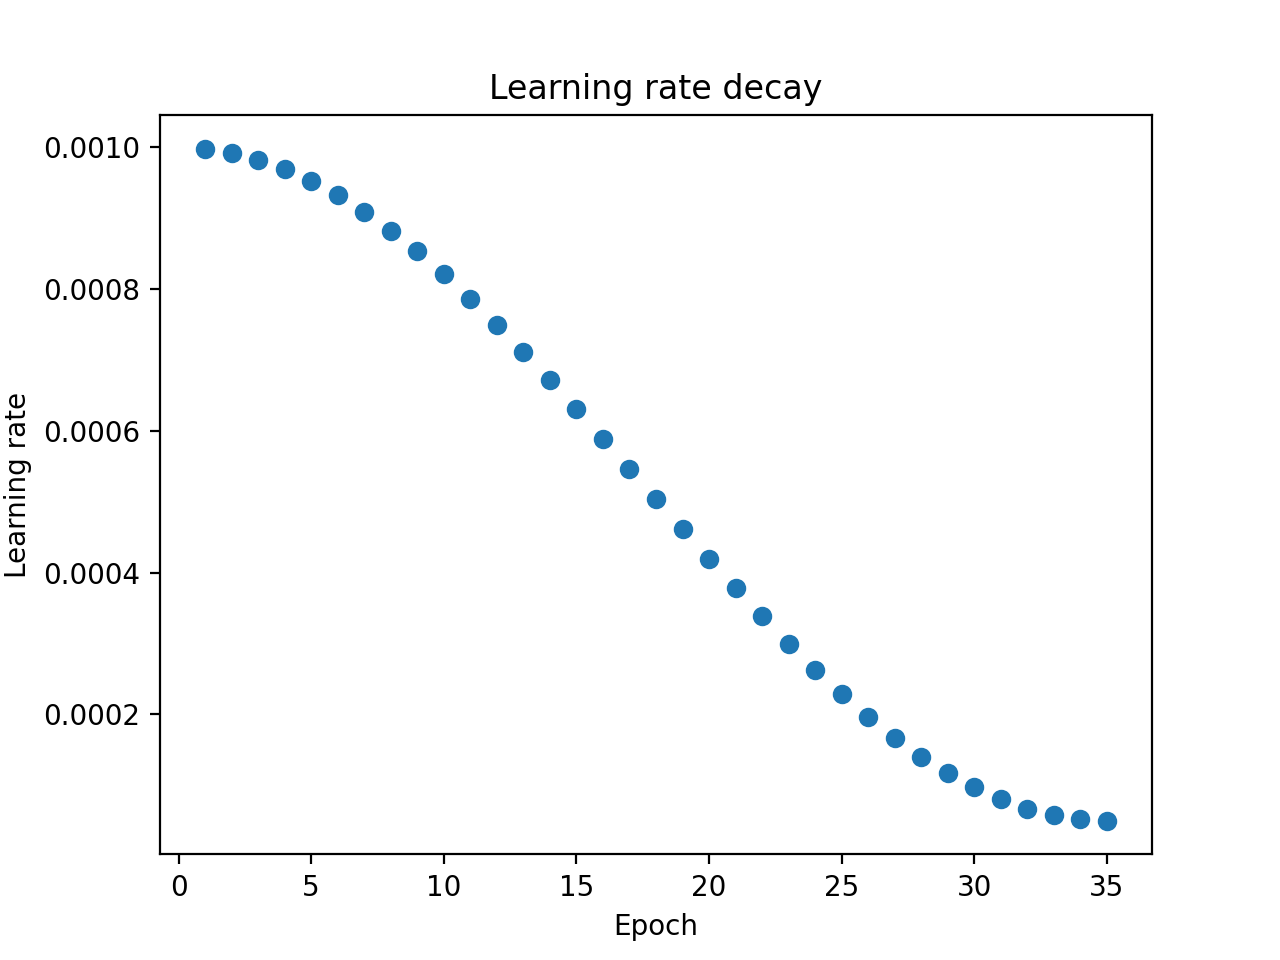
\includegraphics[width=.6\linewidth]{img/LR.png}
	\caption{Exemplary learning rate schedule for 35 epochs applied during training of the detection models.}
	\label{fig:lr_schedule}
\end{figure*}

As described in the ResNeXt paper we load the images and then perform the augmentations necessary to fit the model requirements. To do so, we use a custom dataloader that provides batches of images together with the one-hot encoded ground truth vectors. The augmentation steps done during dataloading include:

\begin{itemize}
	\item Resize the image to have 256 pixels on the shorter side
	\item Perform a $224 \times 224$ crop in the center of the resized image
	\item Normalize the RGB channels in range $0$ to $1$ to have a mean of $R=0.485; G=0.456; B=0.406$ and a standard deviation of $R=0.229; G=0.224; B=0.225$
\end{itemize}

To prevent overfitting during training and essentially enlargen our dataset we also randomly apply additional augmentations such as horizontal flips ($p=0.5$), random blurs ($p=0.3$), random rotations of up to 20° ($p=1$) or random erasing of between 1 and 10 percent of the image area ($p=0.3$).

Since we have somewhat limited hardware resources at our disposal in comparison to large scale compute clusters that are often used for such training tasks by researchers, we also apply a method called \textit{Autocasting} to speed up training and allow us to use larger batch sizes. The basis of Autocasting is the ability to use mixed precision during network training. While most frameworks such as PyTorch usually use 32bit floating point numbers (single precision) for all calculations, it has been shown that performing some operations with 16bit representations (half precision) does not penalize accuracy but provides a large speedup since more data can fit in the most often constrained GPU memory and the also constrained data transfer bandwidth can be used more effectively \autocite{micikevicius_mixed_2018}. The GPUs that we have at our disposal also feature special matrix multiplication hardware that works best with half precision numbers, meaning that we profit from mixed precision training in a significant way. The speedup for the ResNeXt training for example was almost twice as fast as before. The decision whether to perform operations at half precision is made automatically by PyTorch when the model is wrapped in an autocasting decorator.

We train the ResNeXt with a batch size of 32 (like in the original paper) and perform 35 epochs. To calculate the loss we use Binary Cross Entropy but with Logits as recommended for mixed precision training which uses the log-sum-exp trick to improve the numerical stability and avoid loss terms that cannot be represented by half precision \autocite{pytorch_team_automatic_nodate}. The loss numbers for the training and validation loss can be seen in \vref{fig:resnet_loss}. It can be seen that in the end some overfit occurs where the train loss keeps decreasing and the validation loss stays mostly constant or even increases very slightly. In the end we still decided to use the model after 35 epochs since the loss figures are very good and it also evaluates very well as will be shown later in chapter \vref{chapter:eval_resnext}.

\begin{figure*}
	\centering
	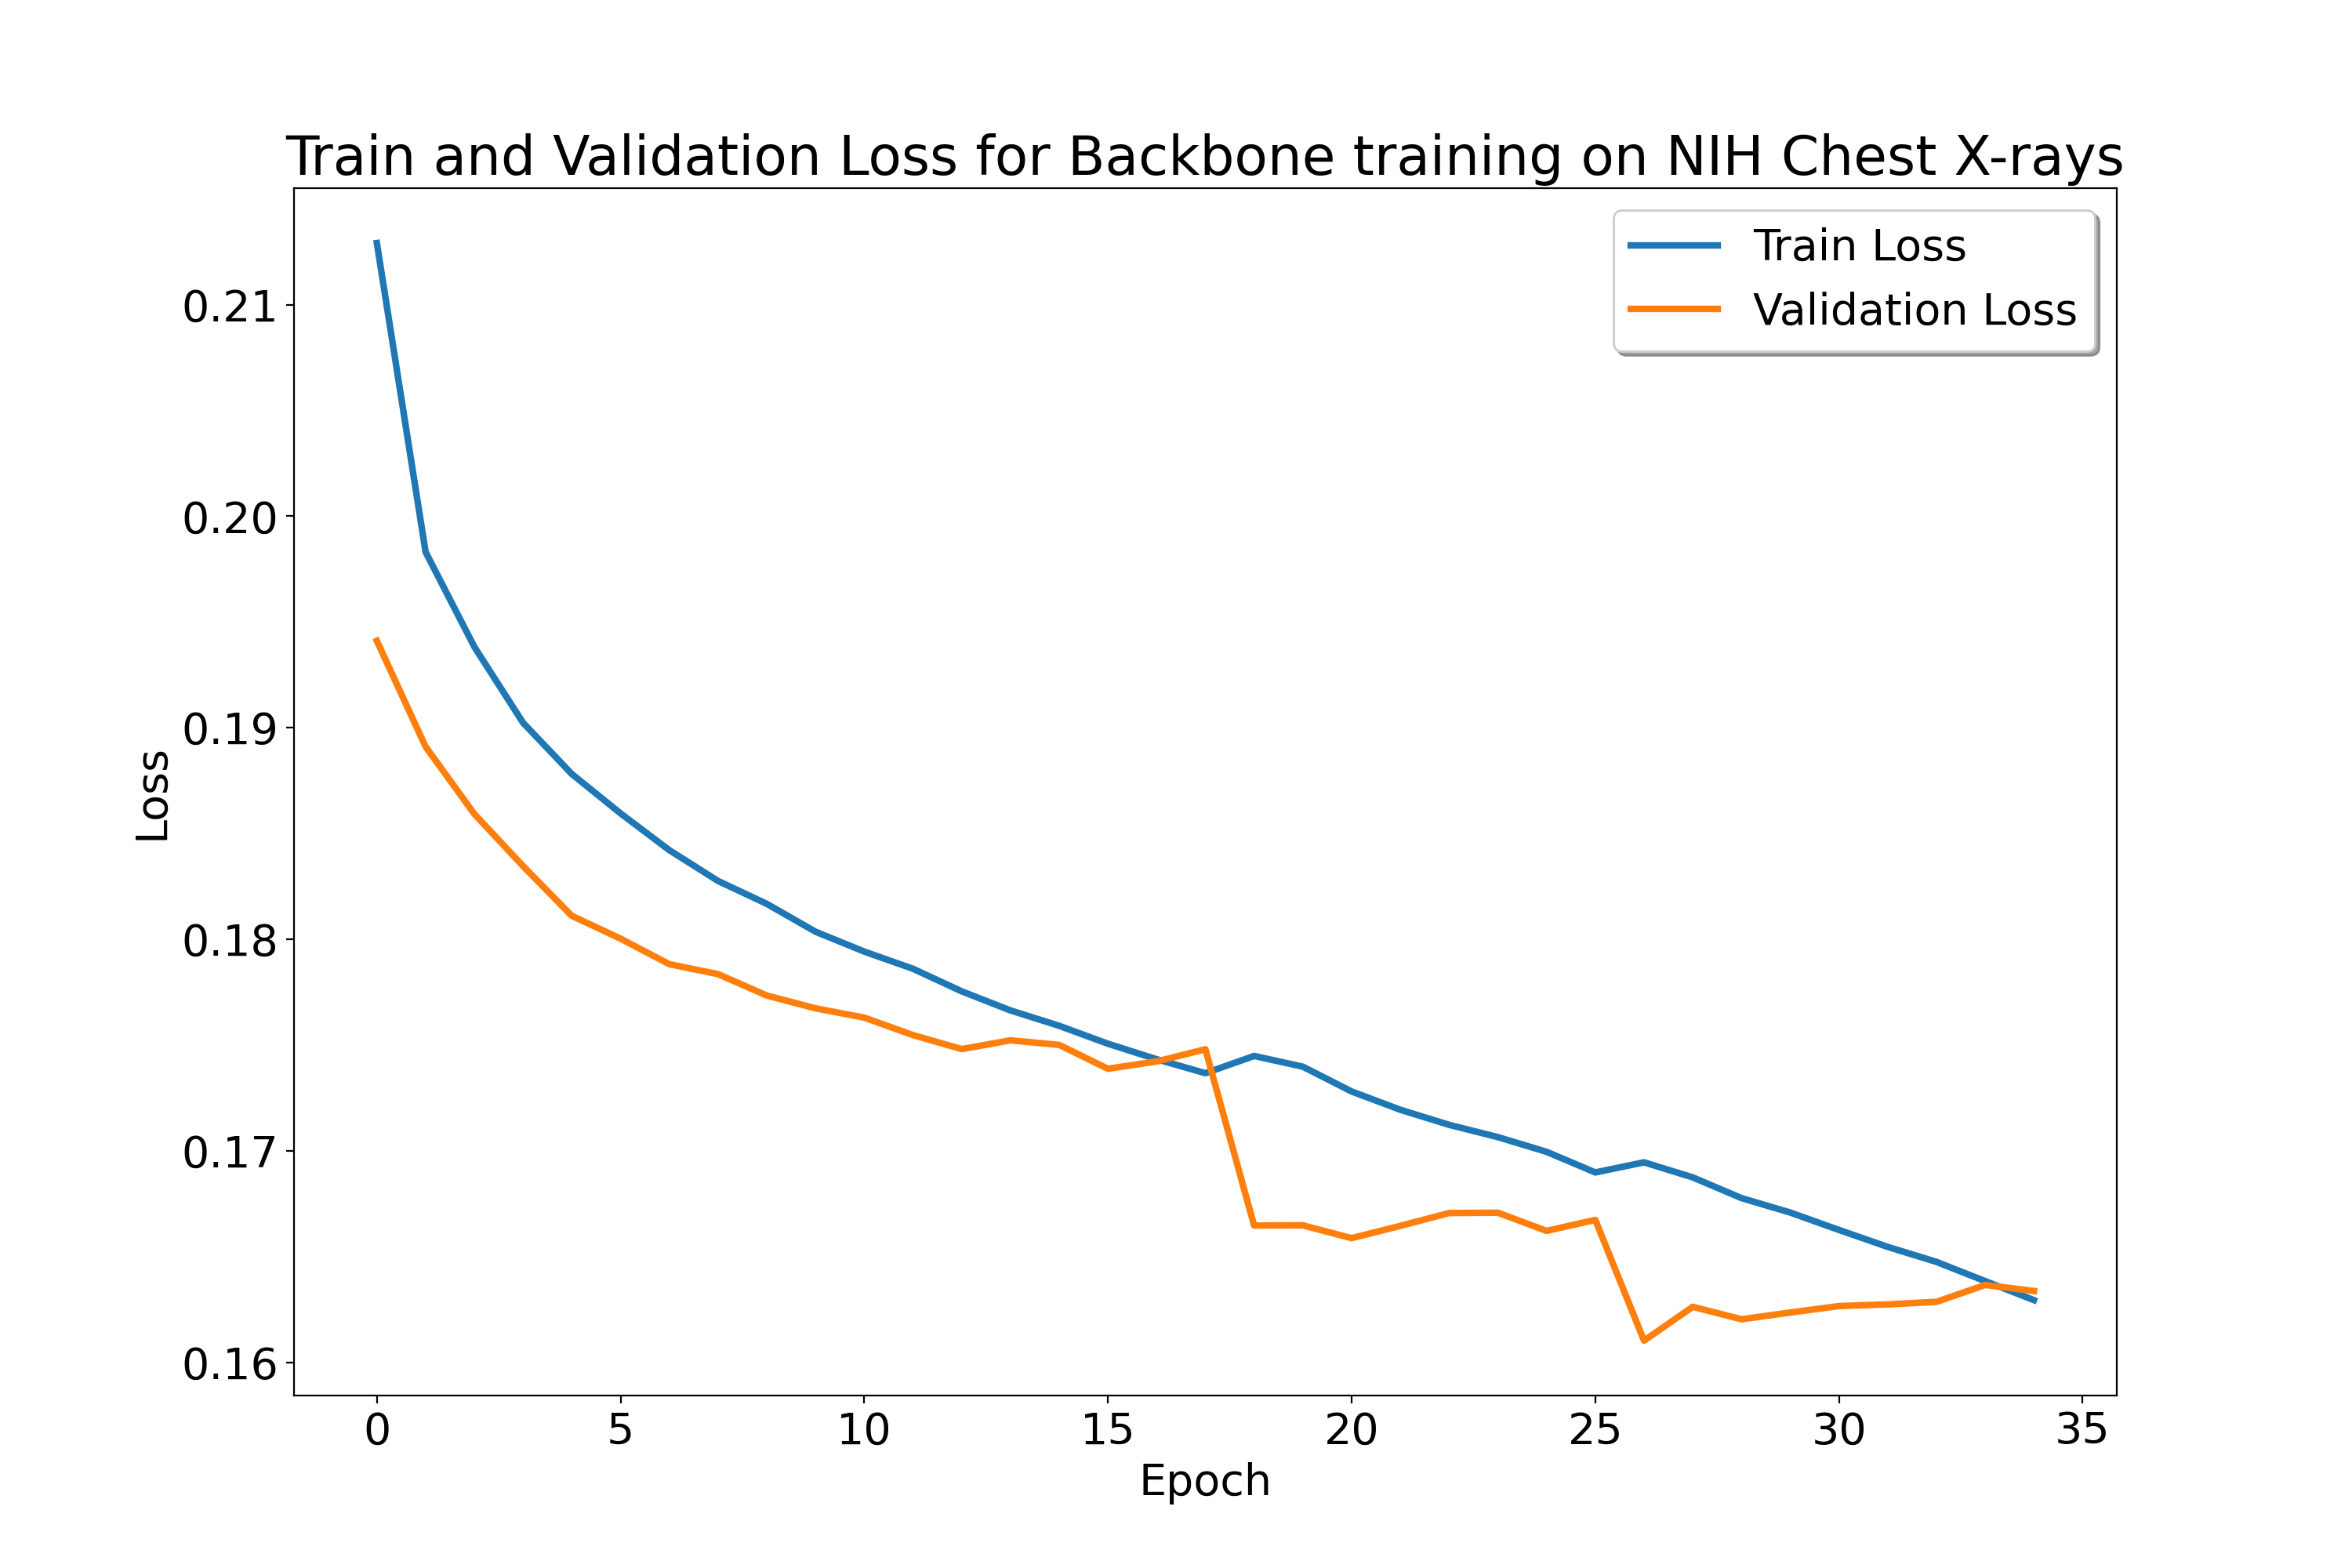
\includegraphics[width=.7\linewidth]{img/loss_backbone_rcnn_35.png}
	\caption{Loss figures of the ResNeXt training}
	\label{fig:resnet_loss}
\end{figure*}

\subsection*{Training of the Faster R-CNN}

With the backbone network trained, we could now train the Faster R-CNN on the actual detection task of predicting where lung opacities are located in a patient's X-ray image. This training shares a lot of optimizations with the backbone network described above. We use the same \ac{SGD} optimizer and learning rate schedule and train for 50 epochs which does not take too long due to the limited number of training images. We also again use autocasting since the speed improvements are too good to leave out.

Due to the limited number of samples available in the SIIM dataset, we now augment the images more extensively to further prevent overfitting. Because we now have bounding boxes in the aforementioned (?) COCO format we also have to apply all augmentations to those too. To also allow the network to better detect small opacities and details we now train with a much larger image size of $512 \times 512$. We also perform random horizontal flips ($p=0.3$), random shifts with rotations of maximum 20° ($p=0.3$), one of random sharpen ($p=0.5$) or blur ($p=0.25$), random brightness and contrast adjustments ($p=0.3$) and random circular cutouts (max. 6; $p=0.3$). During inference however we pass the inputs as $1024 \times 1024$ images to make the results even clearer. As with the backbone net, we also adjust the RGB channels to fit the required mean and standard deviation values.

Due to the much larger input images and network size we can only train the Faster R-CNN with a batch size of 10 and perform validation with a batch size of 6. During training of a Faster R-CNN multiple loss values have to be taken into account since there are the two tasks of classification and bounding box prediction. Detailed loss figures can be seen in figure \vref{fig:rcnn_loss}. As will be evidenced later in chapter \vref{chapter:eval_rcnn_yolo} after 50 epochs there was already some overfit even though the loss numbers look promising.

\begin{figure*}
	\centering
	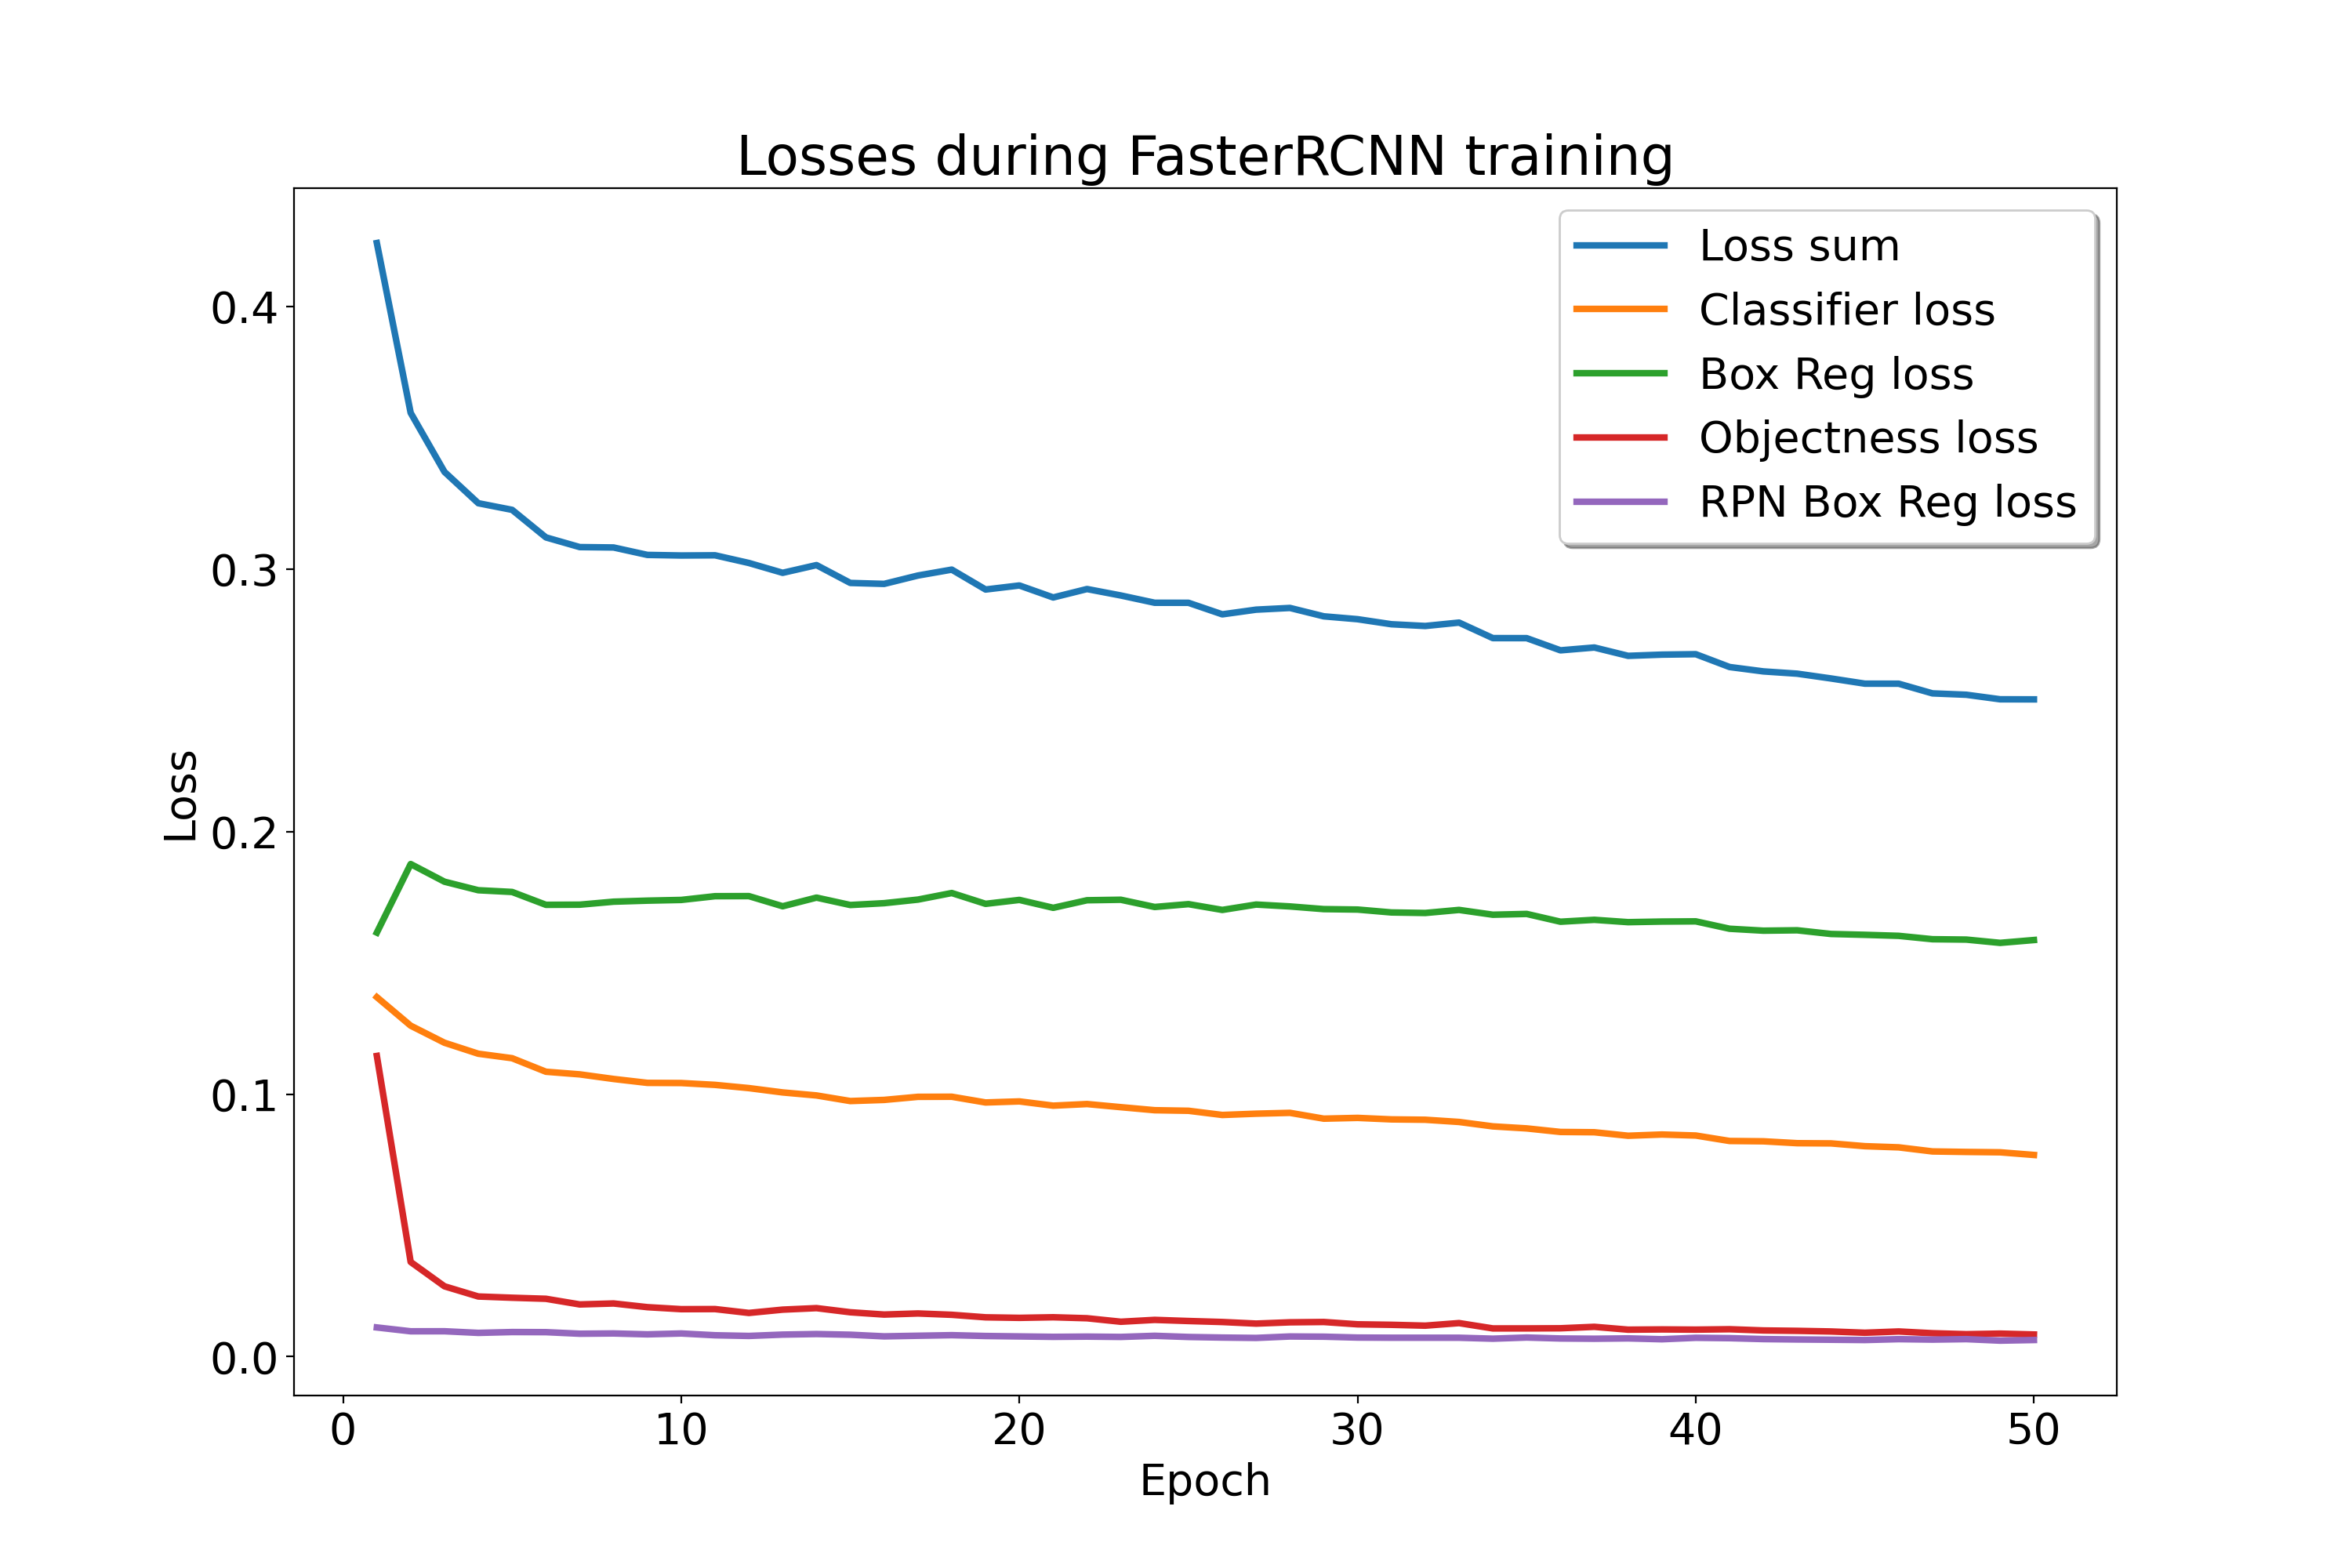
\includegraphics[width=.7\linewidth]{img/loss_fasterrcnn_50.png}
	\caption{Loss figures of the Faster R-CNN training}
	\label{fig:rcnn_loss}
\end{figure*}

Per default a Fast(er) R-CNN uses a smooth L1 loss for the box regression as described in \autocite{girshick_fast_2015} which according to the authors prevents exploding gradients unlike loss functions proposed in earlier R-CNN revisions. However, to try and improve convergence speeds and model accuracy, we also implemented a \ac{CIoU} loss, proposed in \autocite{zheng_enhancing_2021} and described in more detail in section \vref{chapter:yolo}, for the regressor. Unfortunately this did not work at all and the model converged a lot slower than anticipated and sometimes even became a lot worse over time. The reasons for this would need to be investigated further but due to time constraints we had to revert back to using the default smooth L1 loss function which in the end also proved quite capable as will be shown later in the evaluation in section \vref{chapter:eval_rcnn_yolo}.

\section{YOLO}\label{chapter:yolo}
\sectionauthor{Written by Julian Seibel}

The \acl{YOLO} (\ac{YOLO}) model originally proposed in \autocite{yoloOriginal} is an object detector introduced in 2015 by \citeauthor{yoloOriginal}. In contrast to the previous presented Faster \ac{R-CNN}, this model makes its predictions with just a single network evaluation and is therefore called a single-shot detector (hence the name \ac{YOLO}). Unlike in region proposal or sliding window based network architectures, \ac{YOLO} considers the entire image
for predicting which enables the model to implicitly encode context information about the objects. With this, the model is capable of learning the typical shape and size of objects, which objects are likely to occur together and what typical positions objects have in relation to other objects. The initial idea was to provide a object detection network that achieves both, high quality and high inference speed. The authors claim that their \ac{YOLO} model can be up to 1000 times faster than \ac{R-CNN} and up to 100 times faster than Faster \ac{R-CNN}.
Since its initial introduction, the \ac{YOLO} model was adapted in many research problems and has been improved in several follow-up works \autocite{yolov2} \autocite{yolov3} to finally come up with the newest version \textit{V4} \autocite{yolov4}.
In general, a \ac{YOLO} model consist of three main pieces:
\begin{itemize}
	\item The backbone, similar to the Faster \ac{R-CNN}, this is a deep \ac{CNN} that learns image features at different angularities. In their original paper, the authors used a backbone named \textit{Darknet} that is a neural network consisting of 53 convolution
	layers \autocite{yolov3}. However this was substituted with a CSPNet \autocite{wang2020cspnet} since \textit{V4} \autocite{yolov4}
	\item The neck, that is a series of layers which combine features of different convolution layers. Since \textit{V4} the PANet \autocite{tan2020efficientdet} neck is used for this part of the model 
	\item The head, that part consumes the features from the neck and processes them further for the final box, confidence and class prediction
\end{itemize}
The \ac{YOLO} model divides each input image of size $512\times512$ into a $G\times G$ grid, where a grid cell is \enquote{responsible} for an object if it contains the objects' center point. Each grid cell predicts bounding boxes using predefined anchors and corresponding confidence scores that indicate how likely it is that the box contains an object and how well the box fits to the object. For each bounding box a confidence score is predicted using logistic regression. Unlike in \ac{R-CNN}, the \ac{YOLO} model does not predict an offset coordinates for predefined anchors, it rather predicts the location coordinates relative to the center of a grid cell which constraints the coordinates to fall between 0 and 1. This helps the network to learn the parameters more easy. Therefore, the model prediction for a bounding box is a quintuple $(t_x,t_y,t_w,t_h,c)$ consisting of four coordinates and one for the object confidence (also called \enquote{objectness}), where $t_x$ and $t_y$ are the normalized center coordinates of the bounding box. As illustrated in figure \ref{fig:yolo_box}, the model predicts the width and height of the bounding box as offsets from center coordinates of the box and anchors given the offset from the grid cell to the top left image corner ($c_x$,$c_y$) and the anchor width and height ($p_w$,$p_h$) \autocite{yolov2} \autocite{yolov3}.
\begin{figure*}[h!]
	\centering
	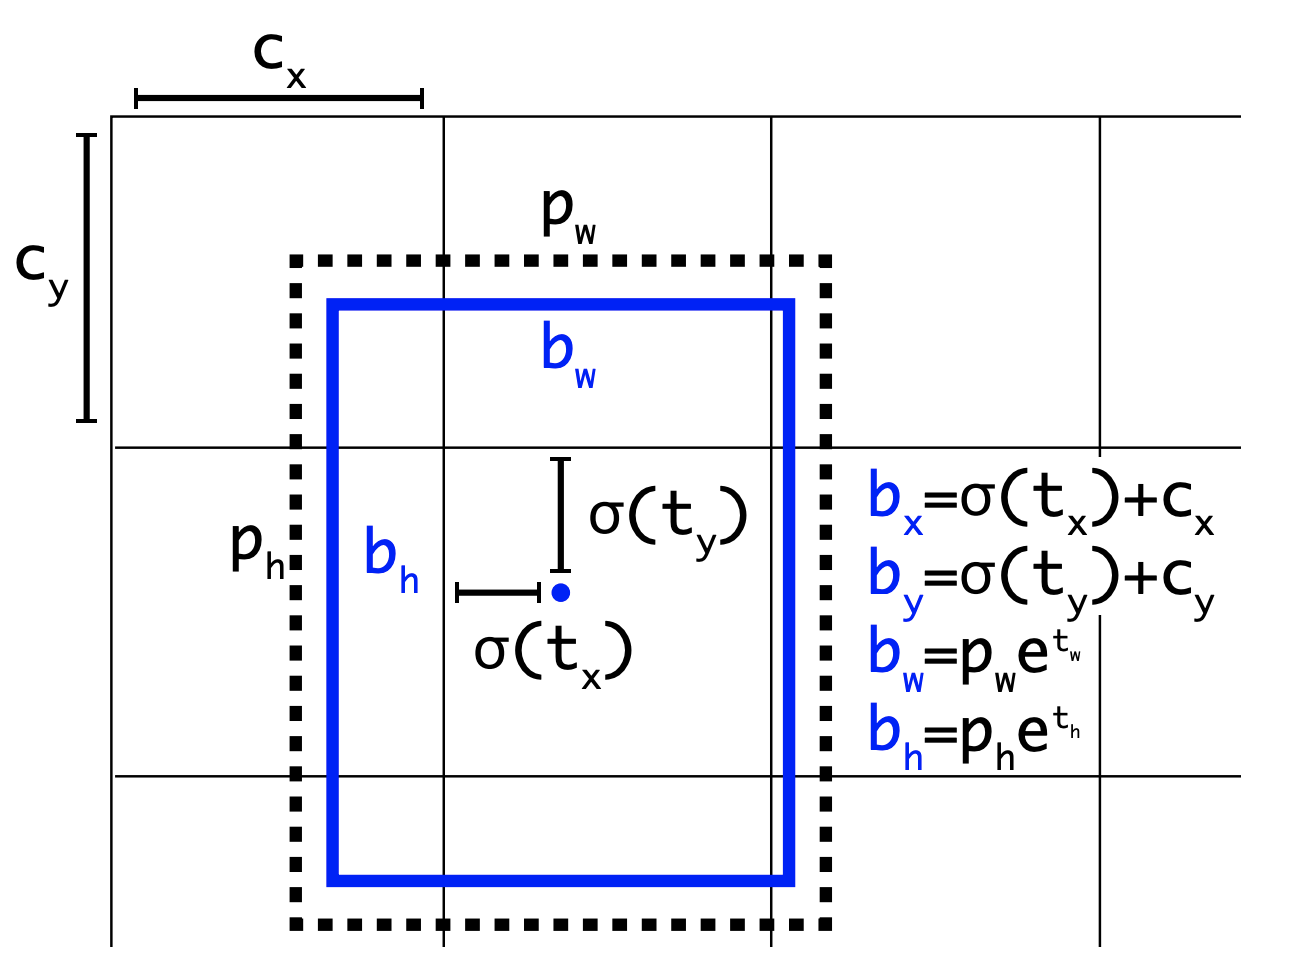
\includegraphics[width=.45\linewidth]{img/boxpred.png}
	\caption{\ac{YOLO} box prediction extracted from \autocite{yolov3}.}
	\label{fig:yolo_box}
\end{figure*}
For each predicted box a class label is assigned using a sigmoid based multi-label classification. The confidence score for a object is then the product of \enquote{objectness} and class confidence to express the probability of a certain class instance appearing in the predicted bounding box and the quality of how well the box fits the object.
The model will produce outputs at different scales and depending on the number of anchors, for each grid cell multiple bounding boxes will be predicted. This often leads to a huge number of predictions per image, which is why non maximum suppression is performed  to filter out boxes that do not meet a certain confidence threshold and that overlap to much in terms of \ac{IoU} (used thrshold of 0.5 in our experiments).


\subsection*{Training of the \ac{YOLO} model}
For our implementation, we decided to use a model provided by \autocite{yolov5} which is called unofficially YOLO \textit{V5} which is based on the YOLO \textit{V4} with some improvements in speed and quality. For our model configuration we used the \textit{yolov5l} model from \autocite{yolov5}.

Similar to \autocite{CoronaDLTransfer} and  \autocite{mangal2020covidaid}, we found that there are not enough data available to achieve state-of-the-art results which is why we use a transfer-learning approach with pretrained weights on the COCO \autocite{coco} dataset, leading to a performance boost in terms of our selected metrics (see \vref{chapter:eval_rcnn_yolo} for further details). Furthermore, we did a second pretraining step, where we used the RSNA pneumonia detection dataset described in \vref{data:rsna}, to adjust the initial COCO-weights in the direction of medical lung images by training the model for 30 epochs. Despite that the objective is different (detecting pneumonia instead of COVID-19), both datasets share many things like the prediction of just one class called \textit{opacity}. We could see an increased performance in the evaluation if we do such a pretraining. The final model is then ultimately trained for 35 epochs on the SIIM COVID-19 data.

As already mentioned in the Faster \ac{R-CNN} training, we did several experiments implementing alternative regression losses for the bounding box predictions. In the \ac{YOLO} paper the authors use a \ac{MSE} regression loss to train the bounding box output. However, as \citeauthor{giou} \autocite{giou} report in their work, there is not a strong correlation between minimizing the \ac{MSE} and improving the \ac{IoU} value. Since a plain \ac{IoU}-based loss would not consider the actual distance of a prediction to a ground truth box, meaning that if there is no intersection, the \ac{IoU} value would be zero and not differentiate between predictions that are close to the ground truth and predictions that are far away from the ground truth.
In addition the authors concern that the evaluation of the model is mostly done using \ac{IoU}-based metrics whereas the training is performed by minimizing a \ac{MSE} loss.

Therefore the authors proposed to use a more appropriate loss they call \ac{GIoU} loss that uses the smallest convex hull of both bounding boxes to encode their relationship also in terms of distance. There exist several extensions like the previously described \ac{CIoU} loss \autocite{zheng_enhancing_2021} or \ac{DIoU} loss \autocite{DIoU}. For our final model, we experienced best results using the \ac{GIoU} loss proposed by \citeauthor{giou}.
The objectness and class confidence predictions were trained using a Binary Cross Entropy with Logits loss. The final loss is then a weighted sum of all the three single losses:
\begin{align}
	\mathcal{L}_{total} = 0.075 * \mathcal{L}_{box} + 0.05 * \mathcal{L}_{class} + 0.75* \mathcal{L}_{objectness}
\end{align} 

For the training process, we used a similar setup like in the Faster \ac{R-CNN} training including a \ac{SGD}-based optimizer with a start learning rate of $lr_{initial} = 0.01$ and momentum of $0.937$, a learning rate scheduling as described in \ref{eq:scheduler} and an input image size of $512 \times 512$. Because of VRAM constrains in our hardware, we could only use a batch size of three (excluding augmentations) but we used a gradient accumulation based on a nominal batch size of $64$, this has the effect that the optimizer and scaler only updates if the nominal batch is over rather than the limited physical batch.
Furthermore we applied $1000$ warm-up iterations, weight decay of 0.0005 following the approach of \autocite{yolov5} and similar to the Faster \ac{R-CNN} approach implemented the training process using \textit{Autocasting} for speed-up. After a forward pass we reduce the amount of possible bounding boxes using non maximum suppression with a confidence threshold of $0.1$ and a \ac{IoU} threshold of $0.2$.
Similar to the Faster \ac{R-CNN} we applied several image transformations as augmentation technique, which include:
\begin{itemize}
	\item Image transformations like flipping up-down (probability of $0.1$) and left-right (probability of $0.5$)
	\item Augmentation of the image and color space using different values for hue, saturation and values in the HSV space
	\item Mixup \autocite{zhang2017mixup} with a probability of $0.5$
\end{itemize}

The losses for the pretraining and actual COVID-19 training are illustrated in figure \ref{fig:yolo_losses}. For the pretraining, we can see a slight increase of the validation loss after about $25$ epochs where we assume this may be caused by overfitting (also visible in the corresponding validation metrics described in \ref{chapter:eval_rcnn_yolo}). The right side of the figure shows the loss and its components for the actual training on the COVID-19 data. It can be seen that also here the loss is decreasing over time, starting already at low level loss values. This and the fact that the losses do not decrease as steep as in the former training is mainly caused by the transfer learning approach using the pretrained weights on the \ac{RSNA} data.
Additionally, the loss graph shows some uncommon pattern which we faced in all our experiments using the \ac{YOLO} model: The validation loss is always smaller than the train loss. Since we did not see any break-in of model performance in terms of metrics measured, we did not follow-up on this, since we could exclude any wrong learning or restrictions of the model. However, such patterns may be caused by:
\begin{itemize}
	\item the validation set being too small
	\item regularization, e.g. dropout that is not active during testing or validation
	\item some shifts due to the time of measurement,the train loss is obtained after every epoch whereas the validation is only measured after a epoch completes. This could cause the mean being pulled from bad performance at the very first iterations of each epochs
	\item some data augmentation effects which is used in the training process but not included in the validation or testing
\end{itemize}

\begin{figure}[h!]
	\centering
	\begin{minipage}{.5\textwidth}
		\centering
		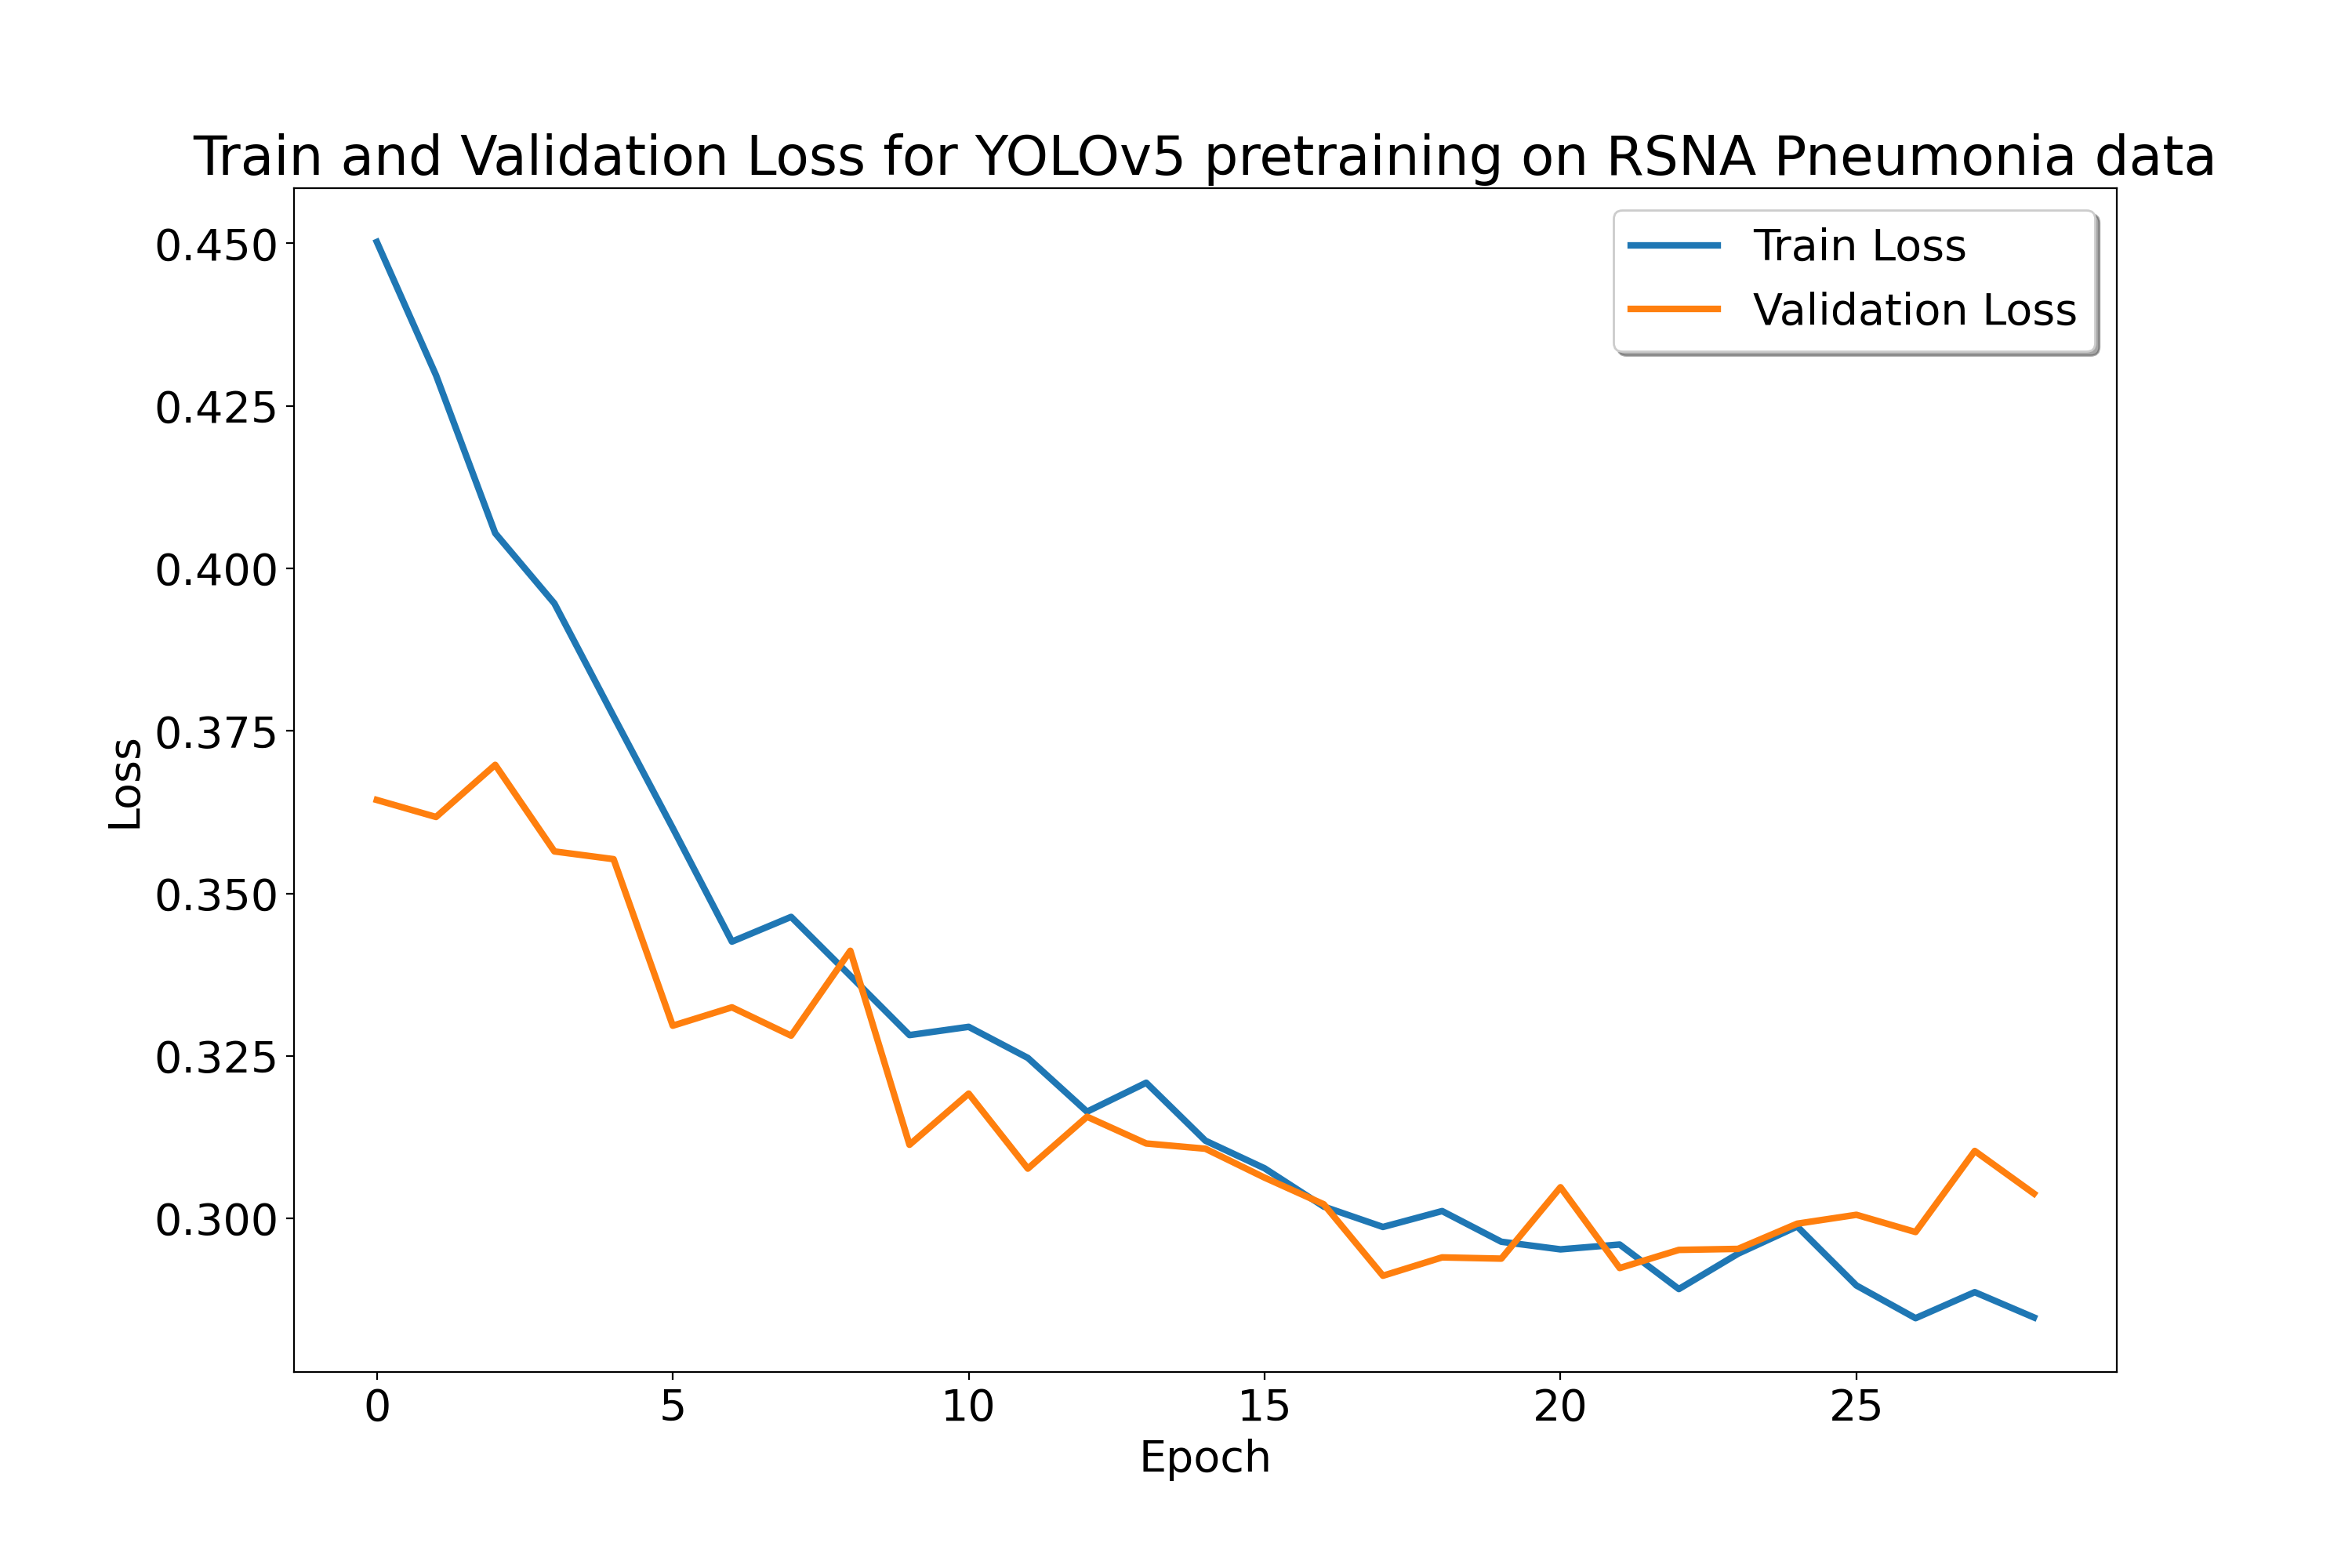
\includegraphics[width=\linewidth]{img/loss_yolo_30.png}
	\end{minipage}%
	\begin{minipage}{0.5\textwidth}
		\centering
		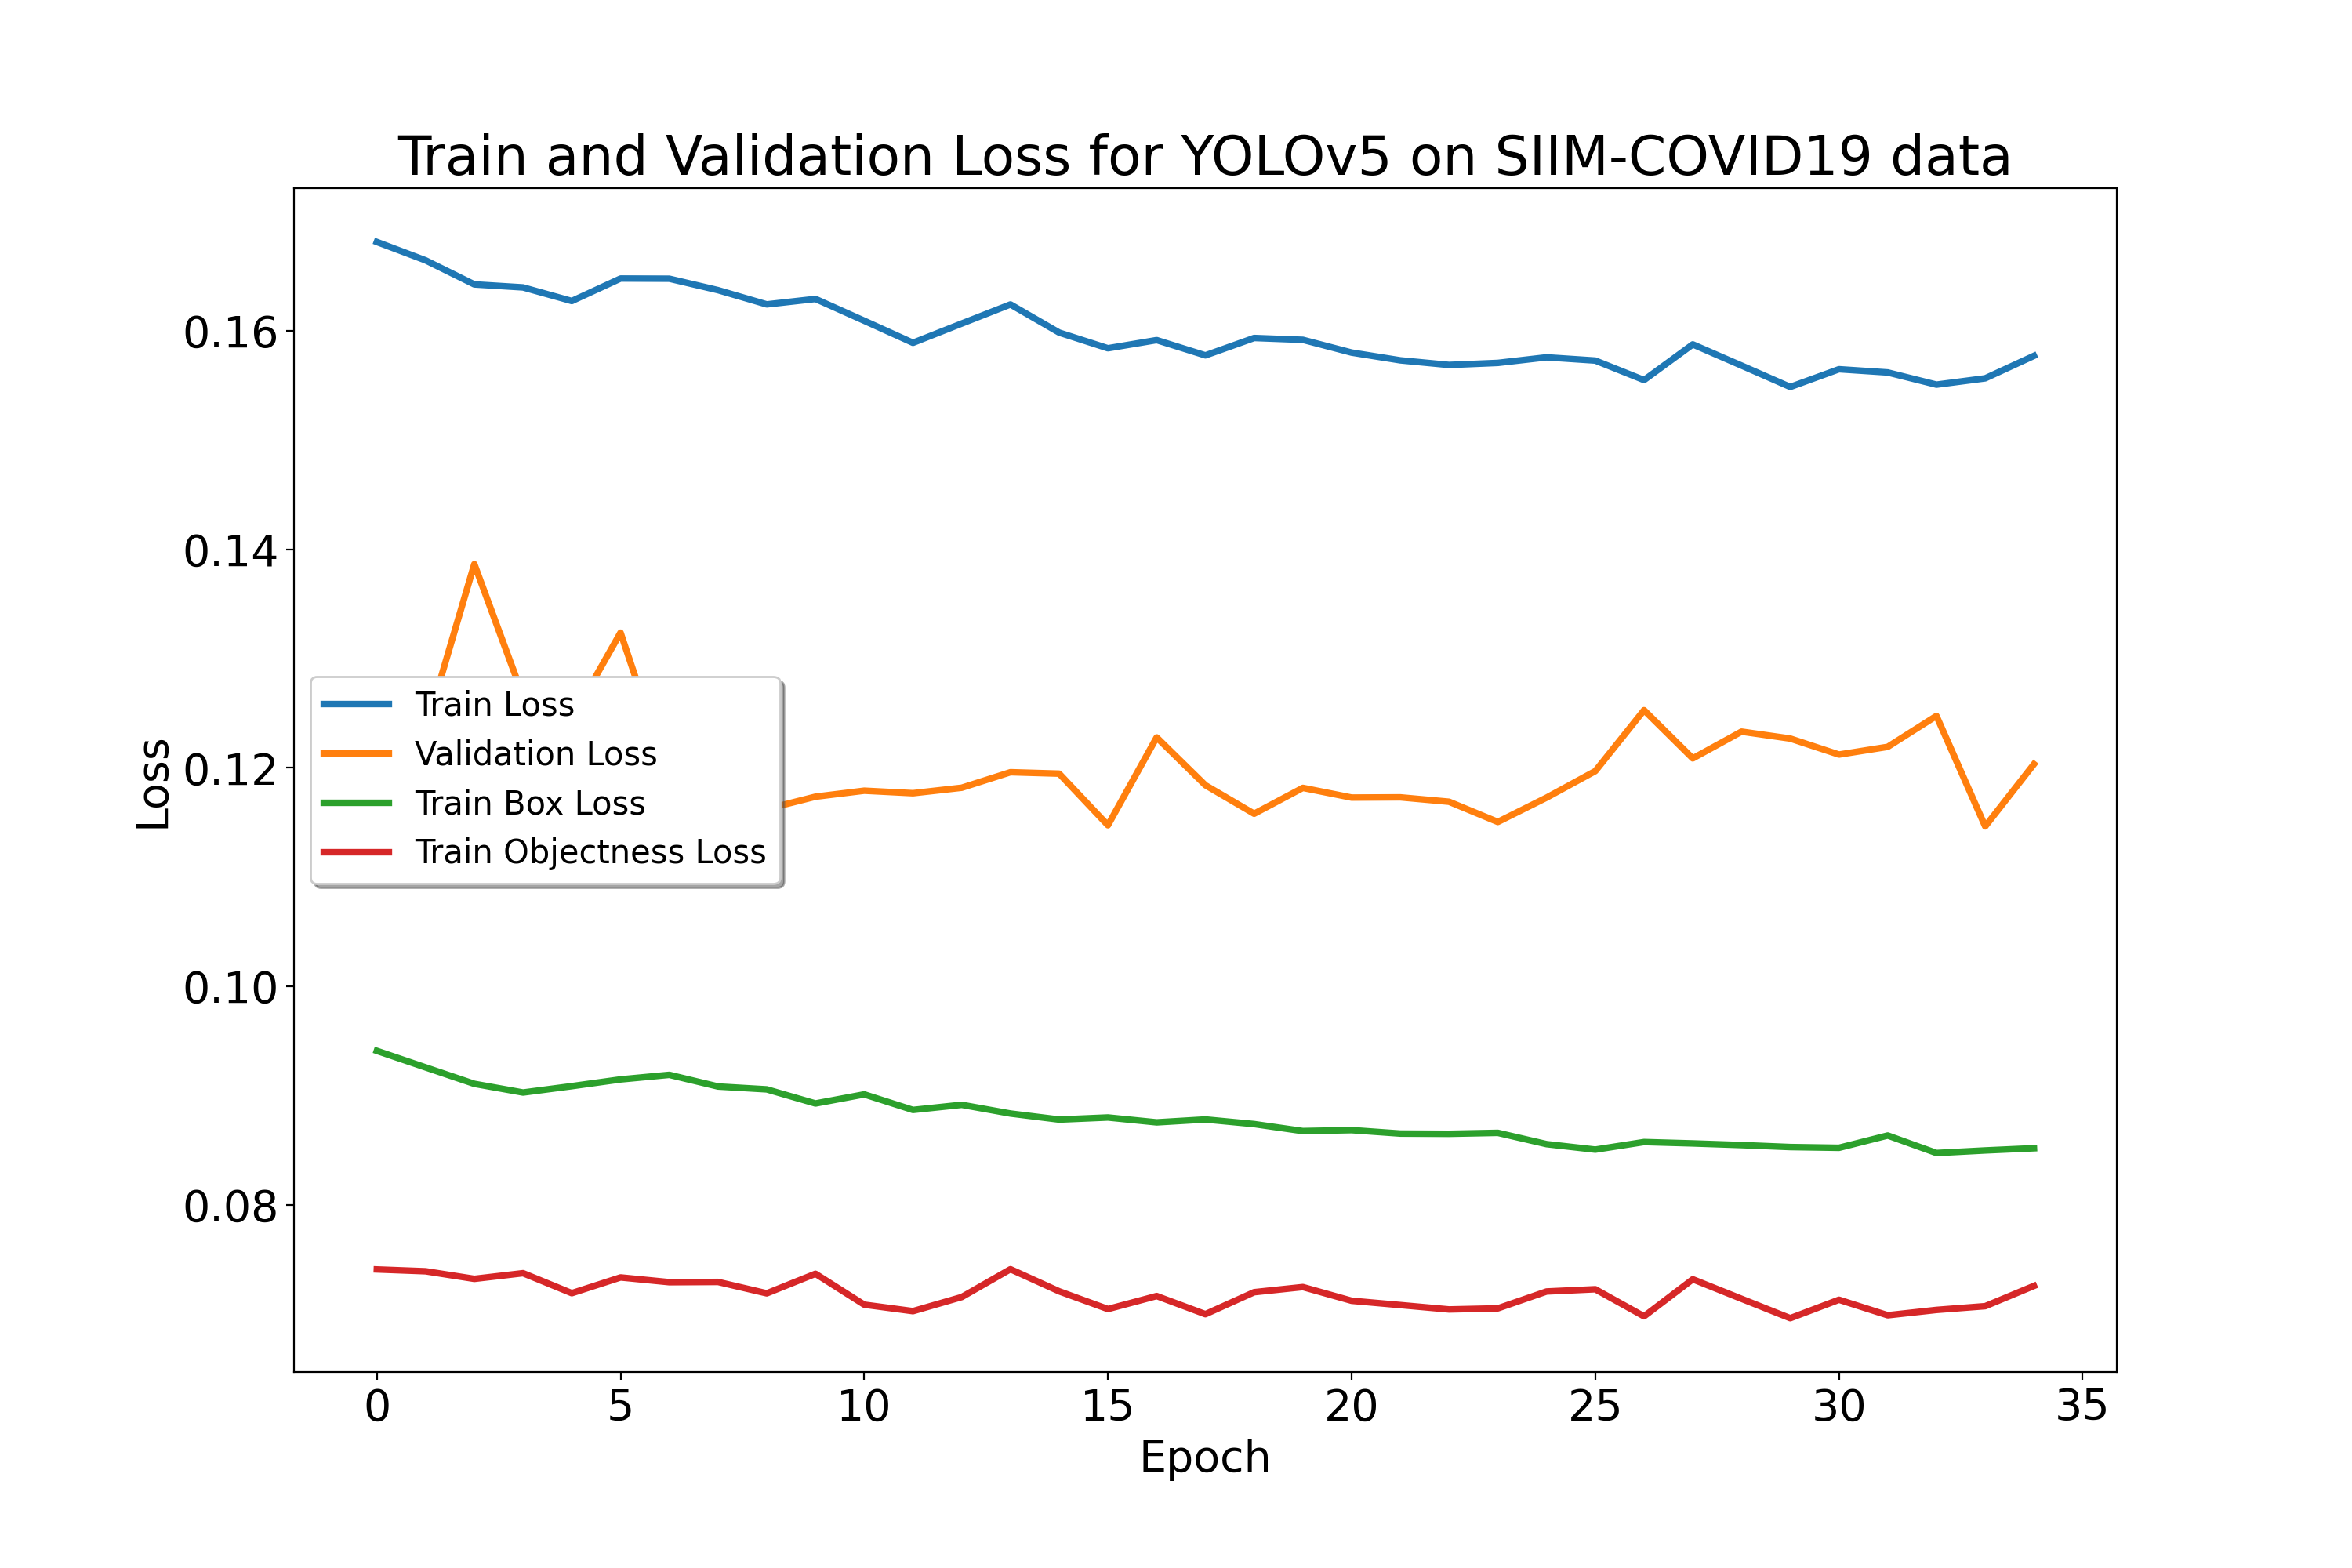
\includegraphics[width=\linewidth]{img/loss_yolo_35_siim_final.png}
	\end{minipage}
\caption{Train and validation loss for the pretraining on the RSNA datset (left) and the SIIM COVID-19 datset (right).}
\label{fig:yolo_losses}
\end{figure}


\section{Combining detections}\label{section:combining_detections}
\sectionauthor{Julian Seibel}
For our final COVID-19 detection, we decided to combine the two described models in an ensemble predictor to combine both advantages of the models and also to create a more stable bounding-box prediction considering both the outputs. For this we created a weighted box fusion following the approach of \citeauthor{weightedBoxFusion} \autocite{weightedBoxFusion}, where we get a final bounding box prediction given the predictions of each model.

Each predicted box is added to a list $B$, that is sorted w.r.t. the corresponding confidence scores. Then two new empty lists are created for boxes clusters $L$ and fused boxes $F$. Each position in $F$ stores the fused box for the corresponding entry $pos$ in $L$. The algorithm then iterates over the predicted boxes in $B$ trying to find a matching box in $F$ based on a \ac{IoU} criteria (e.g. IoU > Threshold, where in our case the threshold was set to 0.55). If no match is found, the box from list $B$ is added $L$ and $F$. In contrast, if a match is found, the box is added to the cluster list $L$ at the corresponding position to the box in $F$. The box coordinates $(x,y)$ and confidence scores $c$ in $F$ will then be recalculated using all boxes accumulated in $L[pos]$ with the fusion equation:
\begin{align}
	c = \frac{\sum_{i=1}^{T}c_i}{T}
\end{align}
\begin{align}
	x_{1,2} = \frac{\sum_{i=1}^{T} c_i * x_{1,2}^i}{\sum_{i=1}^{T} c_i}
\end{align}
\begin{align}
	y_{1,2} = \frac{\sum_{i=1}^{T} c_i * y_{1,2}^i}{\sum_{i=1}^{T} c_i}
\end{align}
Using the confidence scores as weights, predicted boxes with higher confidence naturally contribute more to the fused box.
If all predicted boxes in $B$ are processed, confidence scores in $F$ will be rescaled using the number of predicted bounding boxes $T$ and and the number of participating models $M$:
\begin{align}
	c = c * \frac{min(T,M)}{M}
\end{align}
In our final version, we set the weights for the box fusion $w_{fusion} = (1,1)$ meaning that each model contributes the same to the final prediction.
As fusion-criteria we set an \ac{IoU}-threshold for both predictions to $IoU_{fusion} = 0.55$ which was also the best experienced parameter value described in the original paper \autocite{weightedBoxFusion}. In a last step, we do again non maximum suppression of the fusion boxes to obtain our final ensemble result. 
We did not apply any training process to the ensemble model, but it would be interesting to train the ensemble approach in an end to end fashion. However, we do not have the computational resources available to jointly train both detection models.



\section{Study-Level model}
\sectionauthor{Written by Torben Krieger}


\newpage
% !TEX root =  master.tex
\chapter{Weiterführung}

\newpage
% !TEX root =  master.tex
\chapter{Proposed web application}\label{chapter:webapp}
\chapterauthor{Written by Tobias !}
\newpage
% !TEX root =  master.tex
\chapter{Conclusion}\label{chapter:conclusion}
\chapterauthor{Written by All}

In this project we wanted to create a \ac{CAD} like system that is capable of detecting and classifying COVID-19 infections based on \acl{CXR} images by solving the eponymous Kaeggle challenge. Our solution consists of a multi-stage approach including several deep neural networks to achieve the goal set by the challenge creators. We showed that a \ac{YOLO} and a Faster \ac{R-CNN} are suitable candidates for detecting and localizing COVID-19 regions of interests. Since the dataset required by the challenge is limited, we decided to include the \ac{RSNA} and \ac{NIH} data from previous challenges to pre-train our model weights.
We experienced that the Faster \ac{R-CNN} outperforms the \ac{YOLO} model on our test set, which is also consistent with other work in the field of object detection. However, for our final COVID-19 detection, we created an ensemble model that uses a weighted box fusion of both model outputs ultimately leading to the best results with a \ac{mAP}@$.50$ score of $0.451$. In general we are pleased with the final outcome of the COVID-19 detection performance and think that our work can be used as a solid basis for further research in this area. Due to the limited data we saw some overfitting effects with increased training time, which may be a starting point for further research. This may involve a repetition of our experiments with more data, an ablation study on how the pre-training of both models contribute to the performance or may be a root cause for overfitting effects, a hyper-parameter optimization process or even including more models with different architectures into the ensemble combination. Natural candidates would be for example a RetinaNet \autocite{lin_focal_2018} or a segmentation-based mask R-CNN \autocite{maskRcnn}.
Another interesting extension may include research about an end-to-end train process of the ensemble approach, meaning that there could be an improvement in performance if both single models would be trained together in a joint fashion. However, we only had limited compute resources and time budget which is why we leave this open for further research.

For the classification of COVID-19 infections we were not able to show that our \textit{ResNeXt} model could classify provided images into all the required classes with sufficient performance. However we were able to show that our model is able to decide between COVID-19 typical and negative cases to some extent. Although we were able to overcome the initial overfitting by training the classification layer only, the training did not produce stable and reliable results. The massive overfitting issues show that pre-training is an absolute requirement to solve the classification task of this challenge. To improve the performance either a more extensive pre-training on the NIH dataset could be done, although the pre-training on this dataset also showed already a slight overfitting, or additional pre-trainings on other datasets. There are additional large data sets of \ac{CXR} images publicly available, like the \textit{CheXpert} dataset by \citeauthor{irvin2019chexpert} \autocite{irvin2019chexpert}. On the other hand we could imagine that the limitation of the gradient updates to the classification layer somehow constrains or slows down the training of the model. Thus additional regularization methods should be tried like adding additional dropout layers to the hidden layers of the pre-trained models by redefining the forward path of the pre-trained network part.

In this report we have talked a lot about how different machine learning methods, and in this case computer vision, can help combat the pandemic. Honorably ML researchers and doctors all around the world scrambled to try and help at the start and during the pandemic by providing datasets, studies and models concerning all facets of what to do against the virus, for the infected or for society as a whole. Recently though, doubts have been cast on these efforts, as some studies suggest that machine learning models might not be very effective or in the worst case even dangerous. In a large scale meta study, published in the British Medical Journal, \citeauthor{wynants_prediction_2020} analyze 232 models proposed in 169 studies and find that not a single one is suitable for clinical use but that at least two might be promising with more work \autocite{wynants_prediction_2020}. Another study by \citeauthor{aix-covnet_common_2021} that closely examines 62 studies regarding the topic that we were also working on of identifying COVID-19 infections in patients, comes to the same conclusion that none of them are suitable for clinical use \autocite{aix-covnet_common_2021}. These concerns show that while there has been great effort and a lot of good will in the research community, the processes and studies are not yet as matured as maybe ML researchers and practitioners would like. While most times no harm is done in other areas of ML usage when an error is made, the stakes in the medical field are a lot higher and therefore a lot more care has to be put into every study and ML model that is proposed.

All in all, we liked working on this project. We think that with the global situation around COVID-19, ML may be a key-factor in solving different issues regarding medical image analysis while still keeping the aforementioned concerns in mind. Overall we are very pleased with our results with regards to the detection and localization of opacities. For the classification we expected better results. However we were able to provide solutions for all goals set by the underlying Kaggle Challenge. 

%\input{Kapitel/mitigation.tex}
%	Literaturverzeichnis
\newpage
\ihead{} % Neue Header-Definition
\printbibliography [title=References]


\cleardoublepage

% Der Anhang beginnt hier - jedes Kapitel wird alphabetisch aufgezählt. (Anhang A, B usw.)

\appendix
\ihead{\appendixname~\thechapter} % Neue Header-Definition
% appendix.tex einziehen
%\input{Kapitel/anhangtitle.tex}
%\chapter{Anhang}




% Ehrenwörtliche Erklärung ewerkl.tex einziehen
%% !TEX root =  master.tex

\clearpage
\chapter*{Ehrenwörtliche Erklärung}

% Wird die folgende Zeile auskommentiert, erscheint die ehrenwörtliche
% Erklärung im Inhaltsverzeichnis.

% \addcontentsline{toc}{chapter}{Ehrenwörtliche Erklärung}
Ich versichere hiermit, dass ich die vorliegende Arbeit
 mit dem Thema: \textit{\DerTitelDerArbeit} selbstständig verfasst und keine anderen als die angegebenen Quellen und
Hilfsmittel benutzt habe. Ich versichere zudem,
dass die eingereichte elektronische Fassung mit der gedruckten Fassung übereinstimmt.

\vspace{3cm}
Heidelberg, \today \hfill \DerAutorDerArbeit


\end{document}
